\documentclass[final]{beamer}

% =========================================================
% Preamble - Load all settings from separate files
% =========================================================
% =========================================================
% Packages and Theme Setup
% =========================================================
% TRB poster board: 8 ft (wide) × 4 ft (high) = 96 in × 48 in = 243.84 cm × 121.92 cm
% NOTE: beamerposter expects width/height numbers in cm (it appends 'cm' internally).
\usepackage[orientation=landscape,size=custom,width=243.84,height=121.92,scale=1.0,debug]{beamerposter}
\usepackage{graphicx}
\usepackage{booktabs}
\usepackage{amsmath}
\usepackage{amssymb}
\usepackage{array}
\usepackage{colortbl}
\usepackage{multicol}
\usepackage{tikz}
\usetikzlibrary{shapes,arrows,arrows.meta,positioning,calc}
\usepackage{adjustbox}  % For scaling content to fit fixed containers
\usepackage{pifont}     % For \ding symbols (checkmarks, etc.)
\usepackage{qrcode}     % For QR codes (paper link)
\usepackage{fontawesome5} % For social media icons (LinkedIn, etc.)
\usepackage{enumitem}   % For customizing list environments

% Theme Choice - Using "default" to allow custom headers
\mode<presentation>{\usetheme{default}}

% =========================================================
% Font Settings - Arial-like (Helvetica)
% =========================================================
\usepackage[T1]{fontenc}
\usepackage{helvet}
\renewcommand{\familydefault}{\sfdefault}

% Block title font
% Block title font (section header bars) — tuned for 4×8ft readability.
\setbeamerfont{block title}{size=\fontsize{40}{48}\selectfont,series=\bfseries}

\input{preamble/colors}
% =========================================================
% Custom Headline Template - Using TikZ for reliable positioning
% =========================================================
\setbeamertemplate{headline}{
  \begin{tikzpicture}[remember picture,overlay]
    % Green header background (taller for 4×8ft canvas)
    \fill[HKUGreen] (current page.north west) rectangle ([yshift=-11cm]current page.north east);
    
    % Gold accent line
    \fill[AccentGold] ([yshift=-10.6cm]current page.north west) rectangle ([yshift=-11cm]current page.north east);
    
    % Left column - TRB badge
    \node[anchor=north west, rounded corners=10pt, fill=white, fill opacity=0.15, text opacity=1, inner sep=18pt] 
      at ([xshift=1.2cm,yshift=-1.0cm]current page.north west) {
      \begin{tabular}{c}
        {\color{AccentGold}\fontsize{30}{34}\selectfont\textbf{105TH ANNUAL}}\\[-0.05cm]
        {\color{AccentGold}\fontsize{30}{34}\selectfont\textbf{MEETING}}\\[0.55cm]
        {\color{white}\fontsize{66}{74}\selectfont\textbf{TRB 2026}}\\[0.5cm]
        {\color{white}\fontsize{44}{50}\selectfont Washington, D.C.}\\[0.5cm]
        {\color{white!80}\fontsize{34}{40}\selectfont January 11-15, 2026}
      \end{tabular}
    };
    
    % Center - Title and authors - adjusted position
    \node[anchor=north, white, align=center] at ([yshift=-1.0cm]current page.north) {
      {\fontsize{75}{85}\selectfont \textbf{Repositioning in Bike Sharing Systems with}}\\[0.2cm]
      {\fontsize{75}{85}\selectfont \textbf{Broken Bikes Considering On-site Repairs}}\\[0.65cm]
      {\fontsize{52}{58}\selectfont Runqiu Hu$^{1}$, Jia Cui$^{1}$, W.Y. Szeto$^{1,2,3}$}\\[0.18cm]
      {\fontsize{34}{42}\selectfont $^{1}$Dept. of Civil Engineering, HKU \quad 
      $^{2}$HKU Shenzhen Institute of Research and Innovation \quad 
      $^{3}$GD-HK-Macau Joint Lab for Smart Cities}
    };
    
    % Right column - Journal info
    \node[anchor=north east] at ([xshift=-1.6cm,yshift=-1.0cm]current page.north east) {
      
\includegraphics[height=8cm]{HKU.png}
    };
  \end{tikzpicture}
}

% Custom footline with HKU Green background
\setbeamertemplate{footline}{
  \begin{tikzpicture}[remember picture,overlay]
    % Green footer background - 2cm height
    \fill[HKUGreen] (current page.south west) rectangle ([yshift=3cm]current page.south east);
    
    % Gold accent line at top of footer
    \fill[AccentGold] ([yshift=2.9cm]current page.south west) rectangle ([yshift=3.3cm]current page.south east);
    
    % Left - Personal website
    \node[anchor=west, white] at ([xshift=1cm,yshift=1.55cm]current page.south west) {
      {\fontsize{44}{50}\selectfont \textbf{https://rqhu1995.github.io}}
    };
    
    % Center - University name
    \node[anchor=center, white] at ([yshift=1.55cm]current page.south) {
      {\fontsize{44}{50}\selectfont \textbf{The University of Hong Kong}}
    };
    
    % Right - Email
    \node[anchor=east, white] at ([xshift=-1cm,yshift=1.55cm]current page.south east) {
      {\fontsize{44}{50}\selectfont \textbf{runqiuhu@connect.hku.hk}}
    };
  \end{tikzpicture}
}

% Remove navigation symbols
\setbeamertemplate{navigation symbols}{}


% =========================================================
% Layout Configuration - FIXED GRID (driven by \paperwidth/\paperheight)
% TRB poster (landscape): 8 ft × 4 ft = 243.84cm × 121.92cm
% Header/Footer are fixed; row heights are computed to exactly fill the remaining space.
% =========================================================
\newlength{\headerheight}
% Header needs to read from a distance on a 4×8ft board.
\setlength{\headerheight}{11cm}

\newlength{\rowgap}
\setlength{\rowgap}{0.4cm}

\newlength{\colgap}
\setlength{\colgap}{0.4cm}

\newlength{\contentmargin}
\setlength{\contentmargin}{0.5cm}

% Footer height
\newlength{\footerheight}
% Must cover the full footline drawing height (your accent line reaches 3.3cm).
\setlength{\footerheight}{3.3cm}

% Compute total height available for the two-row grid:
% (paper height) - (header) - (footer) - (two row gaps)
\newlength{\contentheight}
\setlength{\contentheight}{\dimexpr\paperheight-\headerheight-\footerheight-2\rowgap\relax}

% Row heights (2 rows)
\newlength{\rowoneheight}
\setlength{\rowoneheight}{0.5\contentheight}

\newlength{\rowtwoheight}
\setlength{\rowtwoheight}{0.5\contentheight}

% Column 3 (Numerical Studies + Conclusions): give more height to Section 5
\newlength{\colthreerowoneheight}
% Give Section 5 more room on the larger 4×8ft canvas (prevents Section 5 content from overlapping Section 6).
% Use a decimal multiplier to avoid TeX "Dimension too large" overflow in intermediate arithmetic.
\setlength{\colthreerowoneheight}{0.72\contentheight}
\newlength{\colthreerowtwoheight}
\setlength{\colthreerowtwoheight}{\dimexpr\contentheight-\colthreerowoneheight\relax}

% Column width (3 columns with gaps)
\newlength{\colwidth}
\setlength{\colwidth}{0.33\paperwidth}

% Grid debug toggle (set \showgridfalse to hide)
\newif\ifshowgrid
\showgridfalse

% Tight block template so width matches column/grid exactly
% Use explicit ht (height) and dp (depth) for guaranteed consistent title bar height
\setbeamertemplate{block begin}{
  \vskip0pt
  % Taller title bar for 4×8ft readability.
  \begin{beamercolorbox}[wd=\linewidth,ht=2.1cm,dp=0.7cm,leftskip=0.6cm,rightskip=0.6cm]{block title}
    \usebeamerfont*{block title}\insertblocktitle
  \end{beamercolorbox}
  \begin{beamercolorbox}[wd=\linewidth,sep=0.5cm,leftskip=0pt,rightskip=0pt]{block body}
}
\setbeamertemplate{block end}{
  \end{beamercolorbox}
  \vskip0pt
}

% =========================================================
% Document Body - Fixed Grid Layout using TikZ
% =========================================================
\begin{document}
\begin{frame}[t]{}
\begin{tikzpicture}[remember picture, overlay]

    % ---------------------------------------------------------
    % DEBUG: Draw grid borders (red rectangles)
    % ---------------------------------------------------------
    \ifshowgrid
        % Row 1 borders
        \draw[red, line width=1pt] ([xshift=\contentmargin, yshift=-\headerheight-\rowgap]current page.north west)
            rectangle +(\colwidth, -\rowoneheight);
        \draw[red, line width=1pt] ([xshift=-0.5\colwidth, yshift=-\headerheight-\rowgap]current page.north)
            rectangle +(\colwidth, -\rowoneheight);
        % Column 3 uses a custom split (Section 5 taller)
        \draw[red, line width=1pt] ([xshift=-\contentmargin-\colwidth, yshift=-\headerheight-\rowgap]current page.north east)
            rectangle +(\colwidth, -\colthreerowoneheight);

        % Row 2 borders
        \draw[red, line width=1pt] ([xshift=\contentmargin, yshift=-\headerheight-\rowgap-\rowoneheight-\rowgap]current page.north west)
            rectangle +(\colwidth, -\rowtwoheight);
        \draw[red, line width=1pt] ([xshift=-0.5\colwidth, yshift=-\headerheight-\rowgap-\rowoneheight-\rowgap]current page.north)
            rectangle +(\colwidth, -\rowtwoheight);
        \draw[red, line width=1pt] ([xshift=-\contentmargin-\colwidth, yshift=-\headerheight-\rowgap-\colthreerowoneheight-\rowgap]current page.north east)
            rectangle +(\colwidth, -\colthreerowtwoheight);
    \fi
    
    % ---------------------------------------------------------
    % ROW 1: Sections 1, 3, 5 (top row)
    % ---------------------------------------------------------
    
    % Section 1 - Column 1, Row 1
    \node[anchor=north west, inner sep=0] at ([xshift=\contentmargin, yshift=-\headerheight-\rowgap]current page.north west) {
        \begin{minipage}[t][\rowoneheight][t]{\colwidth}
            \setlength{\textwidth}{\colwidth}\setlength{\linewidth}{\colwidth}
            % Section 1: Background, Motivation & Research Gap
\begin{block}{\fontsize{46}{54}\selectfont 1. Background, Motivation \& Research Gap}
    
    {\fontsize{40}{48}\selectfont \textbf{The Challenge:} Bike Sharing Systems (BSS) face critical operational issues:}
    
    \vspace{0.5cm}
    \noindent
    % Left: Two failure images stacked with key facts | Right: Citi Bike chart
    \begin{minipage}[t]{0.54\linewidth}
        \vspace{0pt}
        % Two images side by side
        \begin{minipage}[t]{0.48\linewidth}
            \centering
            \fcolorbox{MediumGray}{white}{%
                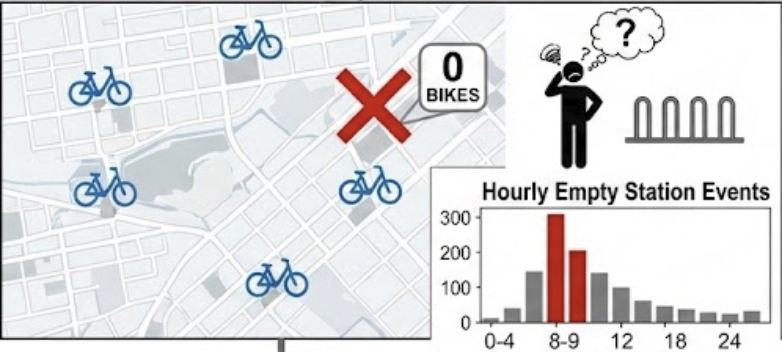
\includegraphics[width=0.94\linewidth,height=12cm,keepaspectratio]{figures/fail_rent.png}%
            }
            \vspace{0.2cm}
            
            {\fontsize{34}{40}\selectfont \textbf{Empty stations} $\rightarrow$ Cannot rent}
        \end{minipage}%
        \hfill
        \begin{minipage}[t]{0.48\linewidth}
            \centering
            \fcolorbox{MediumGray}{white}{%
                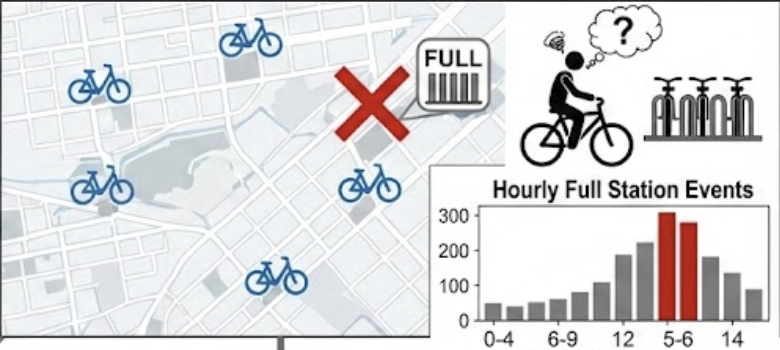
\includegraphics[width=0.94\linewidth,height=12cm,keepaspectratio]{figures/fail_return.png}%
            }
            \vspace{0.2cm}
            
            {\fontsize{34}{40}\selectfont \textbf{Full stations} $\rightarrow$ Cannot return}
        \end{minipage}
        
        \vspace{1.8cm}
        % Key facts as vertical list
        {\fontsize{36}{44}\selectfont
        \begin{itemize}[leftmargin=1.5cm, itemsep=1.5cm]
            \item[•] Barcelona: 12\% severe + 55\% light damage
            \item[•] New York: 2\% need repairs \textit{every day}
            \item[•] Broken bikes occupy docks, reduce inventory
        \end{itemize}}
    \end{minipage}%
    \hfill
    \begin{minipage}[t]{0.43\linewidth}
        \vspace{0pt}
        \centering
        \fcolorbox{MediumGray}{white}{%
            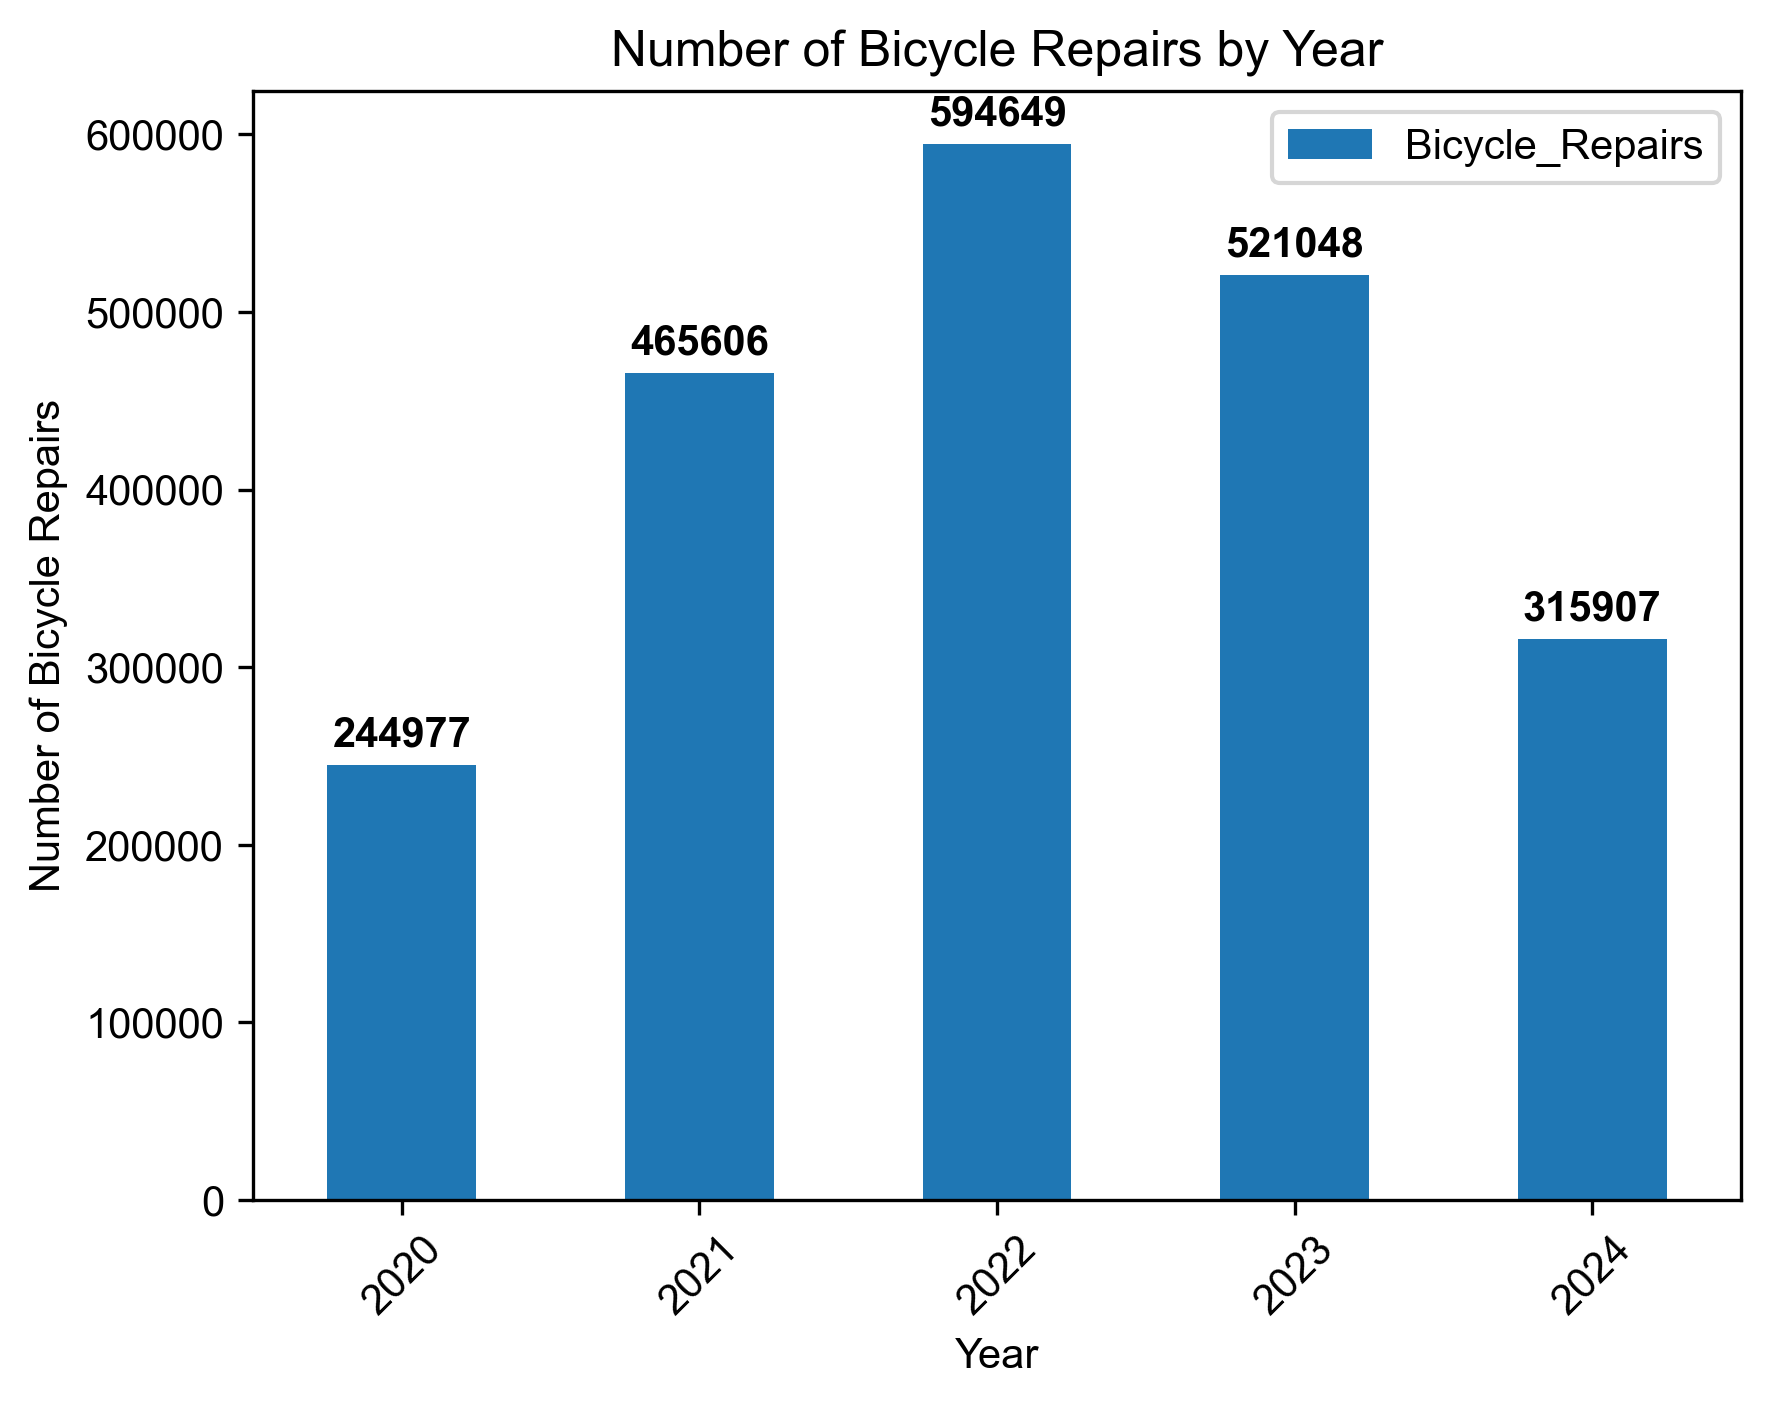
\includegraphics[width=0.95\linewidth,height=19cm,keepaspectratio]{figures/citibike_bicycle_repairs.png}%
        }
        
        \vspace{0.3cm}
        {\fontsize{36}{44}\selectfont Citi Bike: \textbf{21,637 bikes} repaired monthly}
    \end{minipage}
    
    \vspace{0.6cm}
    \hrule
    \vspace{0.6cm}
    
    {\fontsize{40}{48}\selectfont \textbf{Research Gap:} How are broken bikes currently handled?}
    
    \vspace{0.5cm}
    \noindent
    % Two-column comparison with visual emphasis
    \begin{minipage}[t]{0.47\linewidth}
        \vspace{0pt}
        \centering
        \fcolorbox{AlertRed}{white}{%
            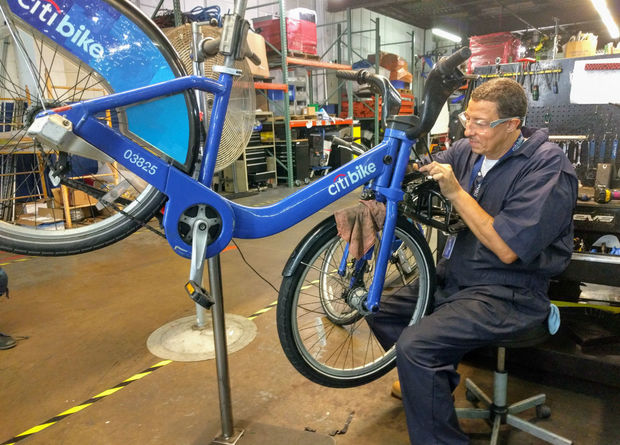
\includegraphics[width=0.94\linewidth,height=16cm,keepaspectratio]{figures/off-site-repair.jpeg}%
        }
        
        \vspace{0.4cm}
        {\fontsize{38}{46}\selectfont \textbf{Off-site Repair} (Depot only)}\\[0.3cm]
        {\fontsize{34}{42}\selectfont \textcolor{AlertRed}{$\blacktriangleleft$ \textbf{Existing studies focus here}}}
    \end{minipage}%
    \hfill
    \begin{minipage}[t]{0.47\linewidth}
        \vspace{0pt}
        \centering
        \fcolorbox{HKUGreen}{white}{%
            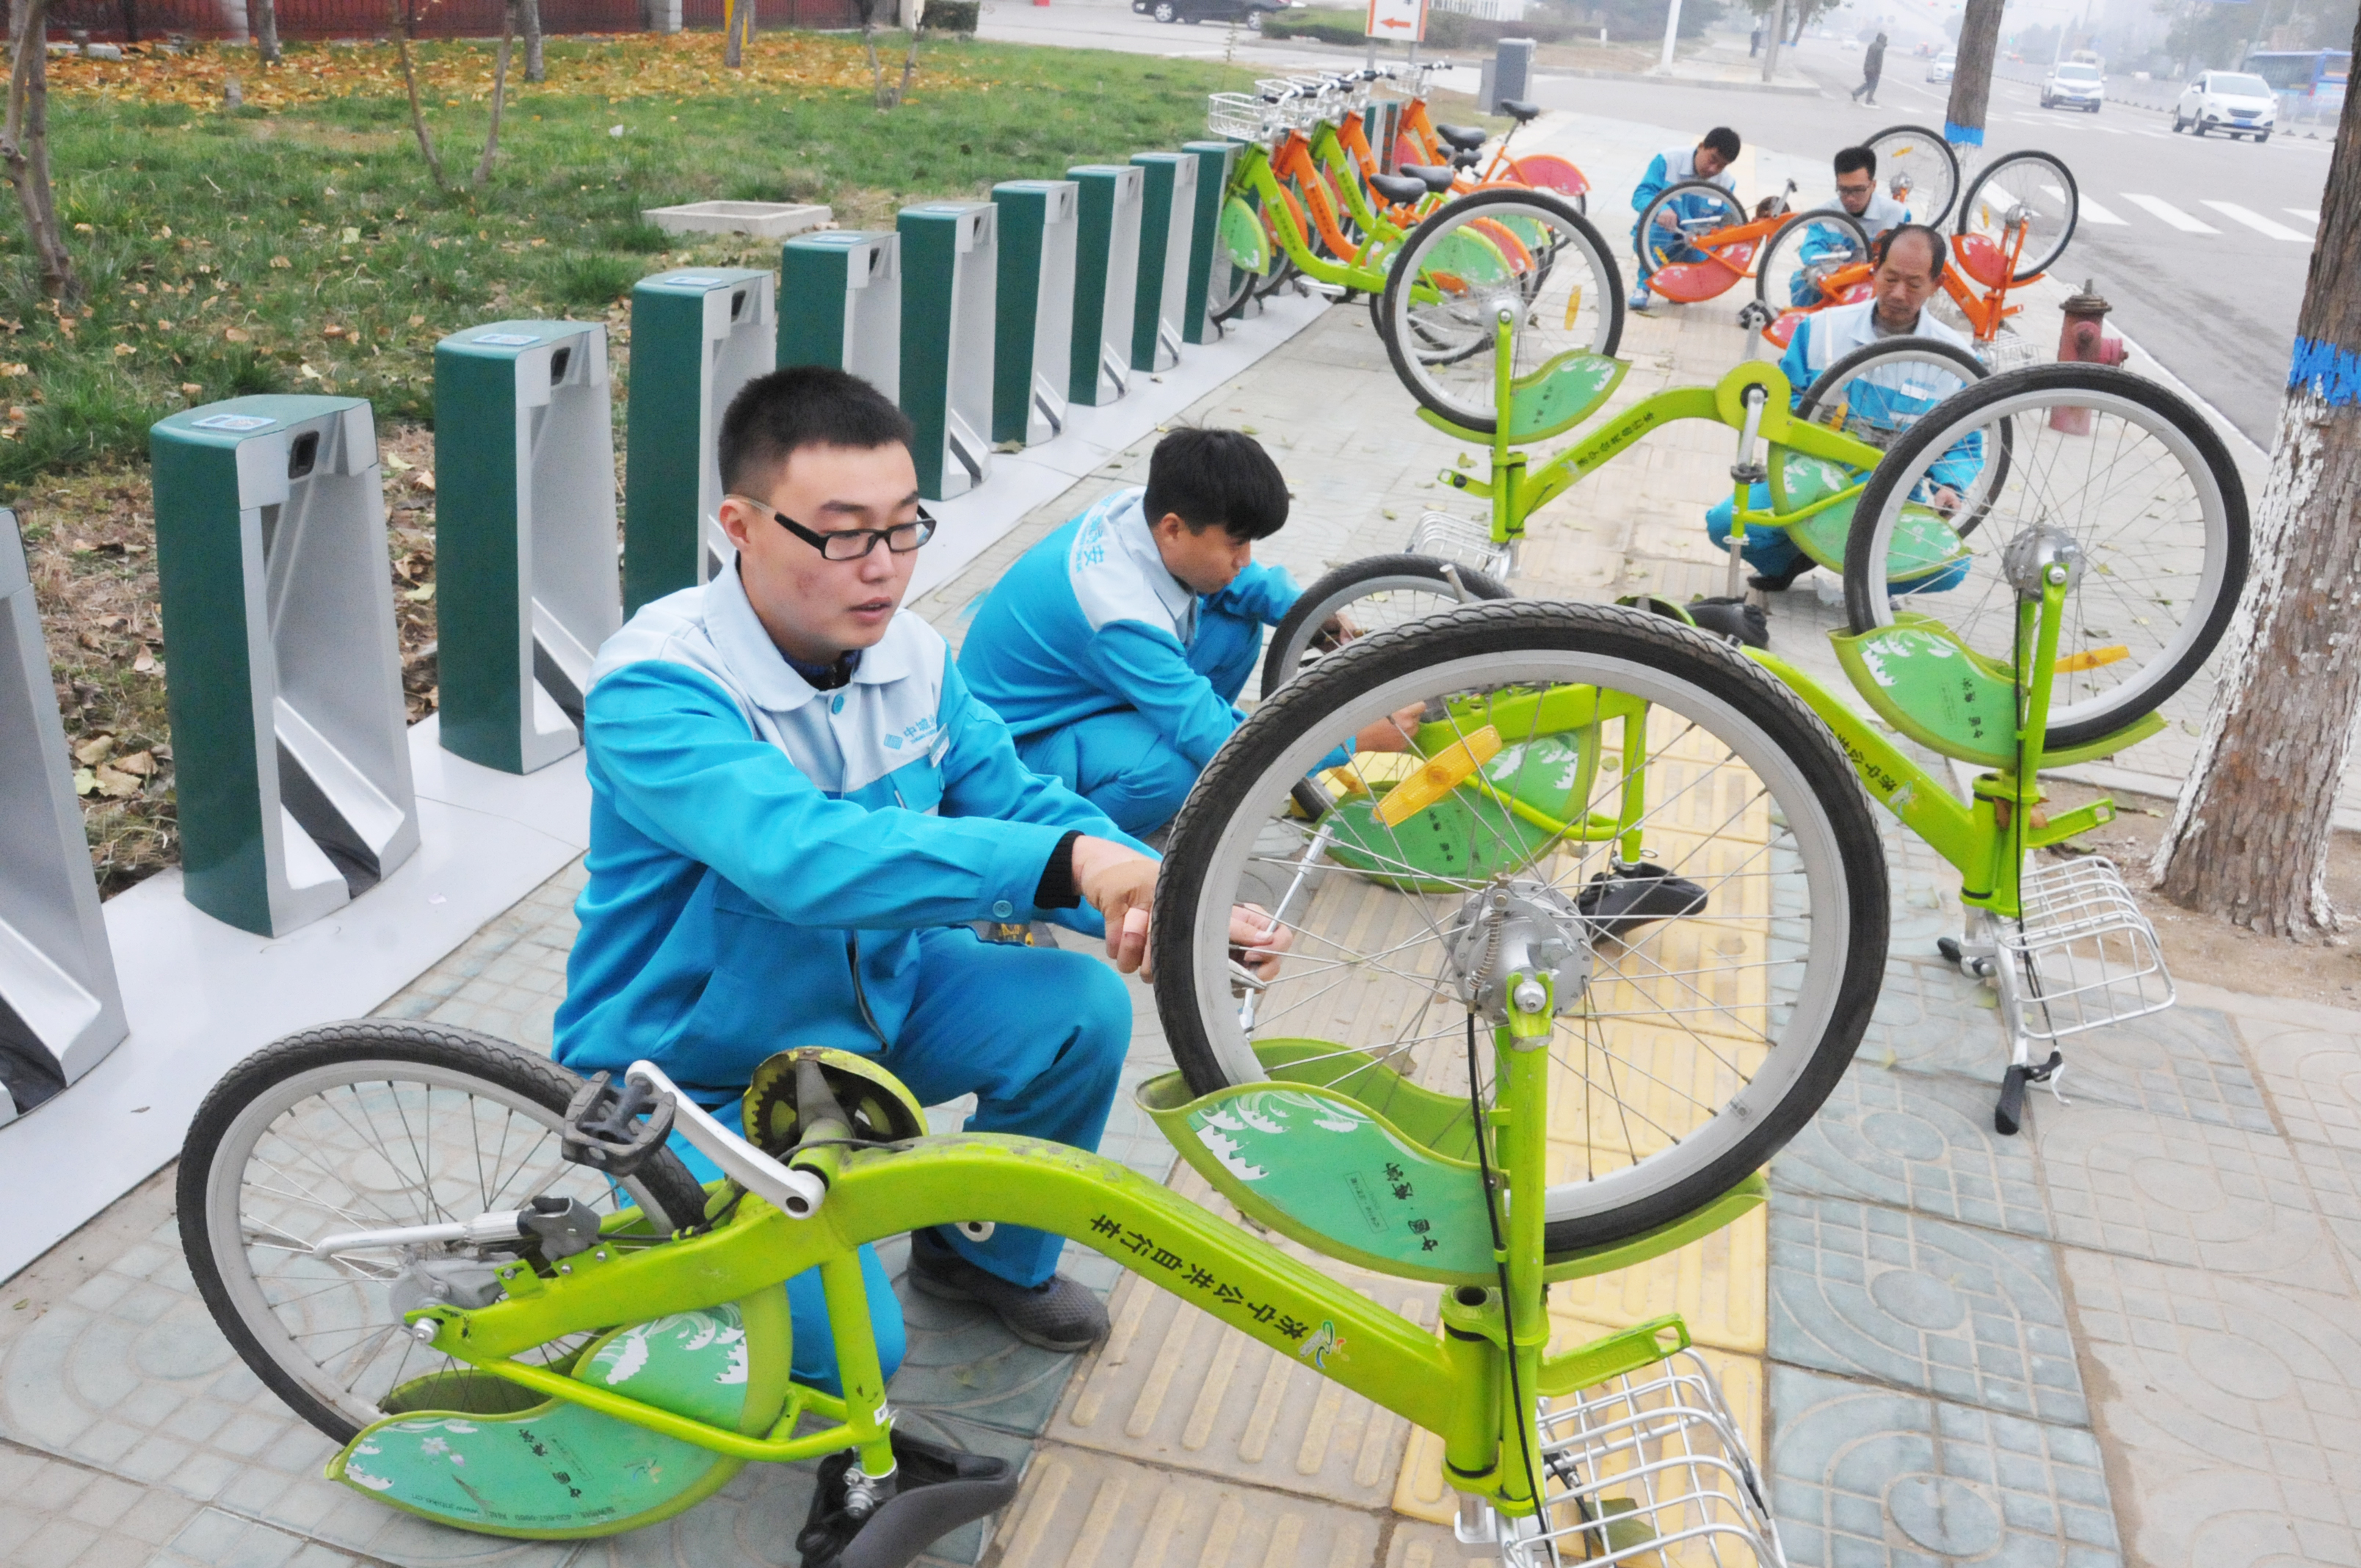
\includegraphics[width=0.94\linewidth,height=16cm,keepaspectratio]{figures/on-site-repair.jpeg}%
        }
        
        \vspace{0.4cm}
        {\fontsize{38}{46}\selectfont \textcolor{HKUGreen}{\textbf{On-site Repair}} (Field)}\\[0.3cm]
        {\fontsize{34}{42}\selectfont \textcolor{HKUGreen}{$\blacktriangleright$ \textbf{Real-world practice}}}
    \end{minipage}
    
    \vspace{0.6cm}
    \colorbox{HKUGreen!15}{\parbox{0.98\linewidth}{\centering
        \vspace{0.4cm}
        {\fontsize{42}{50}\selectfont
        \textbf{Our Innovation:} First to jointly optimize \textbf{Truck-based Repositioning} + \textbf{Repairer-based On-site Repairs}}
        \vspace{0.4cm}
    }}

\end{block}

        \end{minipage}
    };
    
    % Section 3 - Column 2, Row 1
    \node[anchor=north, inner sep=0] at ([yshift=-\headerheight-\rowgap]current page.north) {
        \begin{minipage}[t][\rowoneheight][t]{\colwidth}
            \setlength{\textwidth}{\colwidth}\setlength{\linewidth}{\colwidth}
            % Section 3: Our Approach - Algorithm Framework
\begin{block}{\fontsize{46}{54}\selectfont 3. Our Approach: HGS-ADC with SBC}
    \hspace{0.01\linewidth}    
    % ===== TOP: Algorithm Flowchart + Key Features (SINGLE ROW) =====
    \begin{minipage}[t]{0.56\linewidth}
        \vspace{0pt}
        \centering
        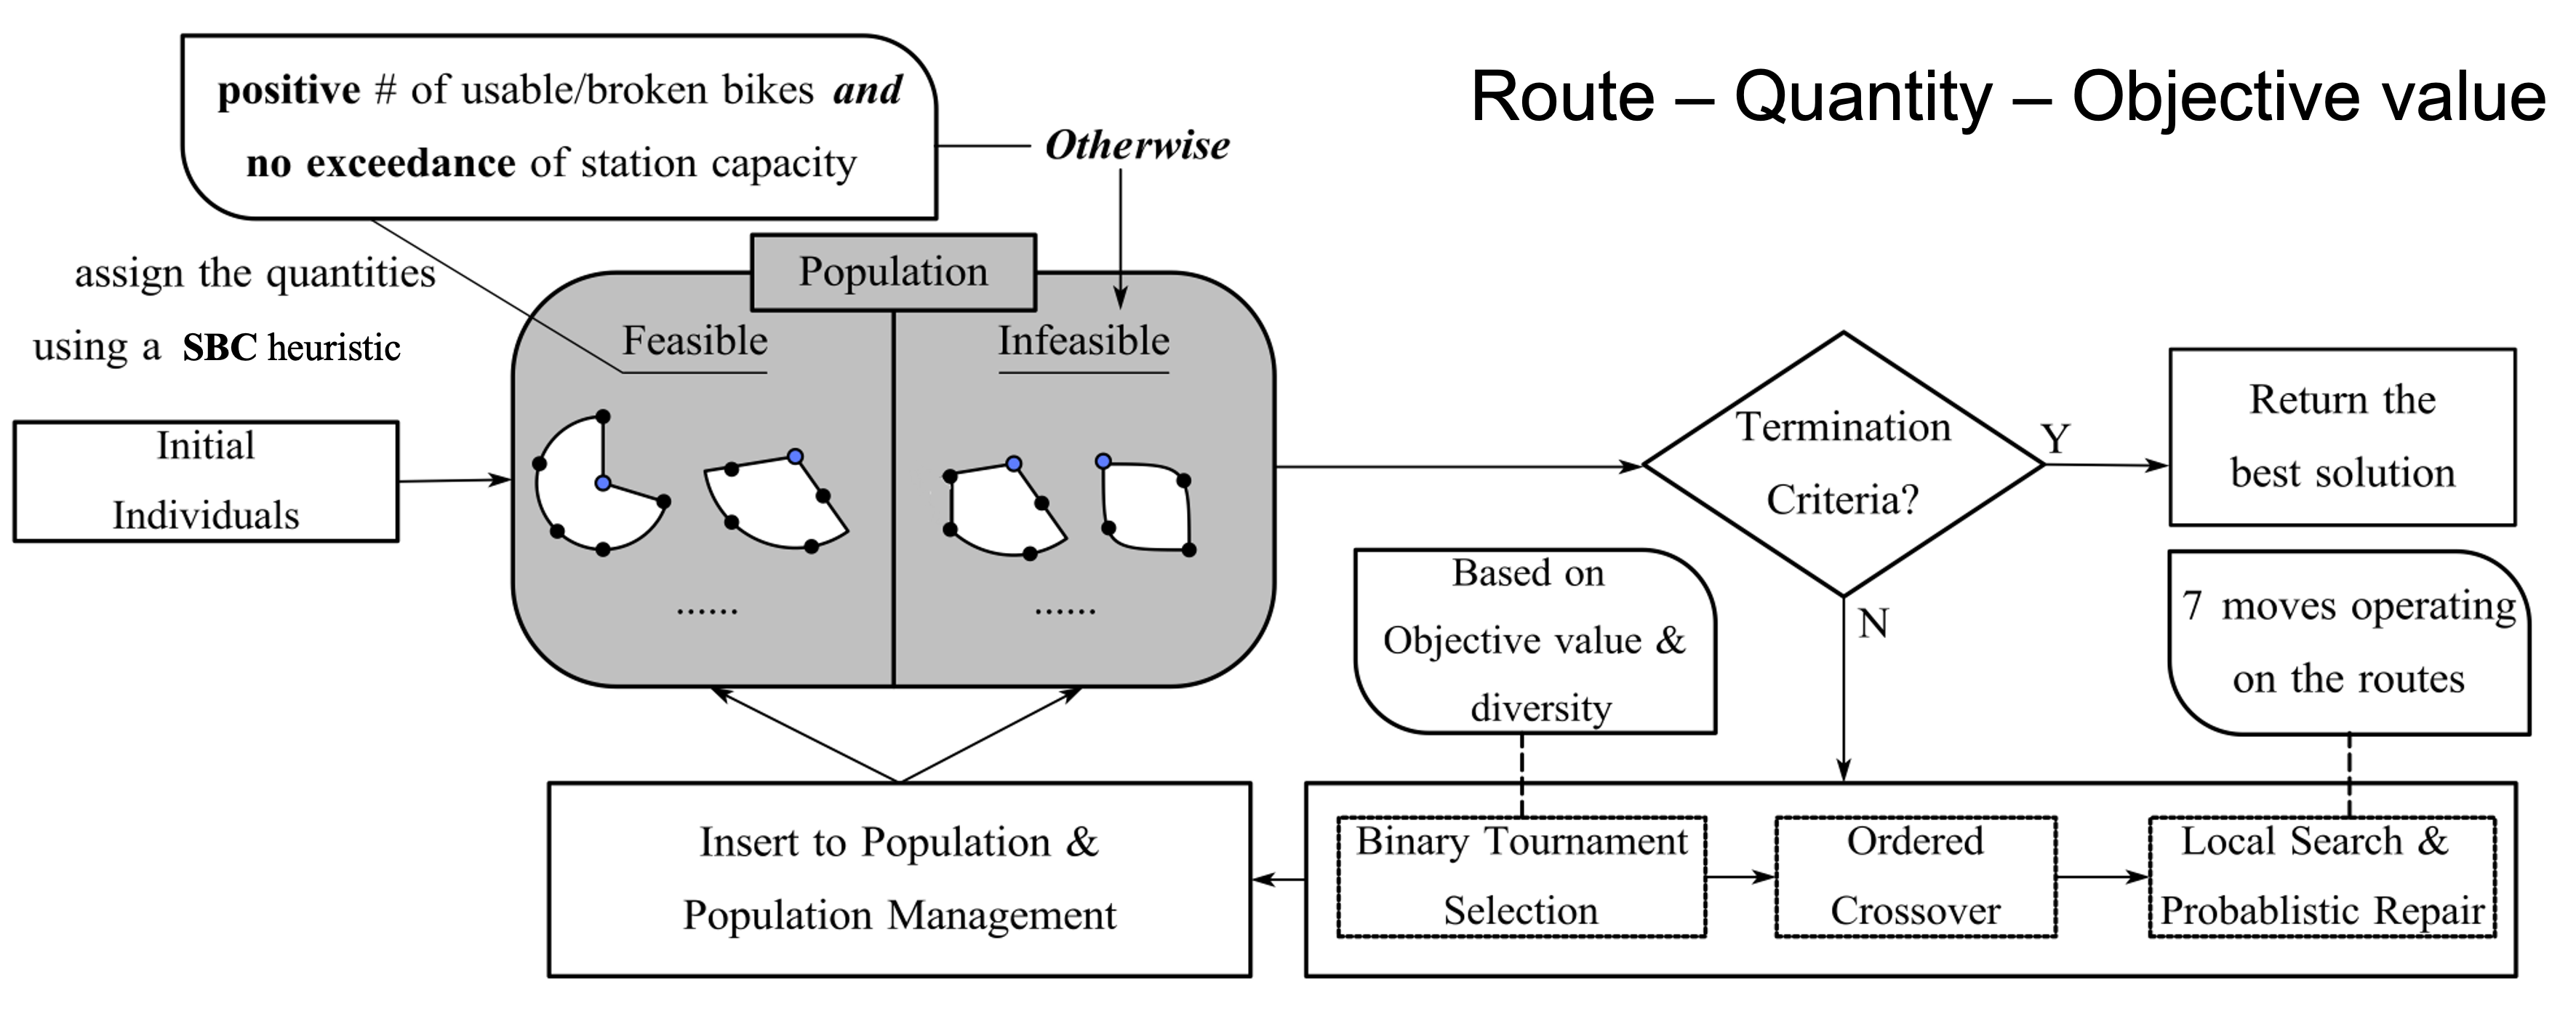
\includegraphics[width=\linewidth]{figures/hgsadc-flowchart.png}
    \end{minipage}%
    \hspace{0.05\linewidth}
    \begin{minipage}[t]{0.46\linewidth}
        \vspace{0pt}
        {\fontsize{42}{50}\selectfont \textbf{Key Features:}}
        
        \vspace{0.8cm}
        
        \fcolorbox{HKUGreen}{HKUGreen!8}{\parbox{0.52\linewidth}{
            \vspace{0.35cm}
            {\fontsize{36}{44}\selectfont \textcolor{HKUGreen}{\ding{202}}~\textbf{Infeasible Population Kept}}\\[0.2cm]
            {\fontsize{32}{40}\selectfont \hspace{0.6cm}Explore beyond feasible boundaries}
            \vspace{0.35cm}
        }}

        \vspace{2.2cm}
        
        \fcolorbox{AccentGold}{AccentGold!8}{\parbox{0.52\linewidth}{
            \vspace{0.25cm}
            {\fontsize{36}{44}\selectfont \textcolor{AccentGold}{\ding{203}}~\textbf{Diversified Search}}\\[0.2cm]
            {\fontsize{32}{40}\selectfont \hspace{0.6cm}Avoid premature convergence}
            \vspace{0.25cm}
        }}
        
        \vspace{2.2cm}
        
        \fcolorbox{AlertRed}{AlertRed!8}{\parbox{0.52\linewidth}{
            \vspace{0.25cm}
            {\fontsize{36}{44}\selectfont \textcolor{AlertRed}{\ding{204}}~\textbf{Adaptive Control}}\\[0.2cm]
            {\fontsize{32}{40}\selectfont \hspace{0.6cm}Dynamic parameter adjustment}
            \vspace{0.25cm}
        }}
    \end{minipage}
    
    \vspace{0.5cm}
    \hrule
    \vspace{0.5cm}
    
    % ===== MIDDLE: Route Decisions + Quantity Assignment =====
    \noindent
    \begin{minipage}[t]{0.42\linewidth}
        \vspace{0pt}
        {\fontsize{40}{48}\selectfont \textbf{\textcolor{HKUGreen}{1. Route Decisions}}}
        
        \vspace{0.25cm}
        {\fontsize{30}{36}\selectfont Local Search: SWAP, 2-opt, Or-opt, Cross-exchange}
        
        \vspace{0.2cm}
        \begin{center}
        \resizebox{0.7\linewidth}{!}{%
        \begin{tikzpicture}[
            station/.style={circle, draw=HKUGreen, fill=white, minimum size=0.9cm, font=\small\bfseries, line width=1.2pt},
            depot/.style={
                rectangle, 
                draw=DarkSlate, 
                fill=white, 
                minimum size=0.8cm, 
                font=\small\bfseries, 
                rounded corners=2pt, 
                line width=1.2pt,
                inner sep=4pt % <--- This leaves margin between text and node border
            },
            truckarrow/.style={-{Stealth[length=2.5mm]}, line width=1.2pt, HKUGreen},
            repairarrow/.style={-{Stealth[length=2.5mm]}, line width=1.2pt, AlertRed, dashed}
        ]
            % Route: Depot -> 3 -> 1 -> 2 -> Depot (greedy visits low-BCRF station first)
            \node[depot] (D) at (0,0) {Depot};
            \node[station] (S3) at (3.5,0) {3};
            \node[station] (S1) at (7,0) {1};
            \node[station] (S2) at (10.5,0) {2};
            
            \draw[truckarrow] (D) -- (S3);
            \draw[truckarrow] (S3) -- (S1);
            \draw[truckarrow] (S1) -- (S2);
            % Truck return: S2 -> down -> left -> up -> Depot
            \draw[truckarrow] (S2.south) -- ++(0,-0.8) -| (D.south);
            
            % Repair D -> S3: from D.north east, up, right, down to S3.north west
            \draw[repairarrow] ([xshift=-0.5cm]D.north east) |- (0.7,0.6) -| (S3.north west);
            % Repair S3 -> S2: from S3.north east, up, right, down to S2.north west
            \draw[repairarrow] (S3.north east) |- (3.9,1.1) -| (S2.north west);
            % Repair S2 -> Depot: from S2.north east, up, left, down to D.north
            \draw[repairarrow] (S2.north east) |- (10.85,1.6) -| (D.north);
        \end{tikzpicture}%
        }
        \end{center}
        
        \vspace{0.4cm}
        \noindent
        {\fontsize{28}{34}\selectfont
        \fcolorbox{HKUGreen}{HKUGreen!10}{\parbox{0.96\linewidth}{\centering\strut\textcolor{HKUGreen}{\textbf{Truck:}} Depot $\to$ 3 $\to$ 1 $\to$ 2 $\to$ Depot}}\\[0.2cm]
        \fcolorbox{AlertRed}{AlertRed!10}{\parbox{0.96\linewidth}{\centering\strut\textcolor{AlertRed}{\textbf{Repairer:}} Depot $\to$ 3 $\to$ 2 $\to$ Depot}}}
    \end{minipage}%
    \hfill
    \begin{minipage}[t]{0.56\linewidth}
        \vspace{0pt}
        {\fontsize{40}{48}\selectfont \textbf{\textcolor{AlertRed}{2. Quantity Assignment}}}~~{\fontsize{30}{36}\selectfont \textit{The Hard Problem!}}
        
        \vspace{0.3cm}
        
        {\fontsize{32}{40}\selectfont
        \renewcommand{\arraystretch}{1.6}
        \begin{tabular}{@{}l|>{\centering\arraybackslash}p{0.24\linewidth}>{\centering\arraybackslash}p{0.24\linewidth}>{\centering\arraybackslash}p{0.24\linewidth}@{}}
            & \textbf{Station 1} & \textbf{Station 2} & \textbf{Station 3} \\
            \hline
            \rowcolor{HKUGreen!10} \textcolor{HKUGreen}{\textbf{Truck}} & $u_1^+, u_1^-, b_1{=}?$ & $u_2^+, u_2^-, b_2{=}?$ & $u_3^+, u_3^-, b_3{=}?$ \\
            \rowcolor{AlertRed!10} \textcolor{AlertRed}{\textbf{Repairer}} & $r_1{=}?$ & --- & $r_3{=}?$ \\
        \end{tabular}
        \renewcommand{\arraystretch}{1.0}}
        
        \vspace{0.2cm}
        {\fontsize{28}{34}\selectfont
        $u^+$: usable bikes loaded~~$u^-$: usable bikes unloaded~~$b$: broken bikes loaded~~$r$: broken bikes repaired}
        
        \vspace{0.8cm}
        \fcolorbox{AccentGold}{AccentGold!15}{\parbox{0.96\linewidth}{
            \vspace{0.2cm}
            {\fontsize{36}{44}\selectfont Each station has \textbf{different sensitivity} to inventory changes}\\[0.15cm]
            {\fontsize{36}{44}\selectfont \textbf{\ding{52} Solution: SBC Allocation with BCRF}}
            \vspace{0.2cm}
        }}
    \end{minipage}
    
    \vspace{0.5cm}
    \hrule
    \vspace{0.5cm}
    
    % ===== BOTTOM: BCRF Explanation =====
    {\fontsize{40}{48}\selectfont \textbf{BCRF: Benefit-Cost Ratio Function}}
    
    \vspace{0.1cm}
    \hspace{0.03\linewidth}
    \begin{minipage}[t][0.98\height][t]{0.28\linewidth}
        \vspace{0pt}%
        \fcolorbox{AccentGold}{AccentGold!15}{\parbox{0.97\linewidth}{%
            \vspace{0.15cm}
            \centering{\fontsize{32}{38}\selectfont \textbf{Stn 1:}~~\textbf{Moderate}}\\[0.65cm]
            \hspace{0.03\linewidth}%
            \begin{minipage}[c]{0.38\linewidth} 
                {\fontsize{30}{36}\selectfont $21.5{-}8.4{=}13.1$}\\[0.08cm]
                {\fontsize{30}{36}\selectfont $\Rightarrow \mathbf{24}$ bikes}
            \end{minipage}%
            \hfill
            \begin{minipage}[c]{0.54\linewidth}
                \raggedleft
                {\fontsize{30}{36}\selectfont $\text{BCRF}{=}\dfrac{13.1}{24}{=}\mathbf{0.55}$}
            \end{minipage}
            \hspace{0.03\linewidth}
            \vspace{0.15cm}
        }}\\[0.2cm]
        \fcolorbox{AlertRed}{AlertRed!15}{\parbox{0.97\linewidth}{%
            \vspace{0.15cm}
            \centering{\fontsize{32}{38}\selectfont \textbf{Stn 2:}~~\textbf{High}}\\[0.65cm]
            \hspace{0.03\linewidth}%
            \begin{minipage}[c]{0.38\linewidth}
                {\fontsize{30}{36}\selectfont $156.8{-}18.2{=}138.6$}\\[0.08cm]
                {\fontsize{30}{36}\selectfont $\Rightarrow \mathbf{44}$ bikes}
            \end{minipage}%
            \hfill
            \begin{minipage}[c]{0.54\linewidth}
                \raggedleft
                {\fontsize{30}{36}\selectfont $\text{BCRF}{=}\dfrac{138.6}{44}{=}\mathbf{3.15}$}
            \end{minipage}
            \hspace{0.03\linewidth}
            \vspace{0.15cm}
        }}\\[0.2cm]
        \fcolorbox{HKUGreen}{HKUGreen!15}{\parbox{0.97\linewidth}{%
            \vspace{0.15cm}
            \centering{\fontsize{32}{38}\selectfont \textbf{Stn 3:}~~\textbf{Low}}\\[0.65cm]
            \hspace{0.03\linewidth}%
            \begin{minipage}[c]{0.38\linewidth}
                {\fontsize{30}{36}\selectfont $7.7{-}0.8{=}6.9$}\\[0.08cm]
                {\fontsize{30}{36}\selectfont $\Rightarrow \mathbf{41}$ bikes}
            \end{minipage}%
            \hfill
            \begin{minipage}[c]{0.54\linewidth}
                \raggedleft
                {\fontsize{30}{36}\selectfont $\text{BCRF}{=}\dfrac{6.9}{41}{=}\mathbf{0.17}$}
            \end{minipage}
            \hspace{0.03\linewidth}
            \vspace{0.15cm}
        }}
    \end{minipage}%
    \hfill
    \begin{minipage}[t][0.98\height][t]{0.70\linewidth}
        \vspace{0pt}%
        \centering
        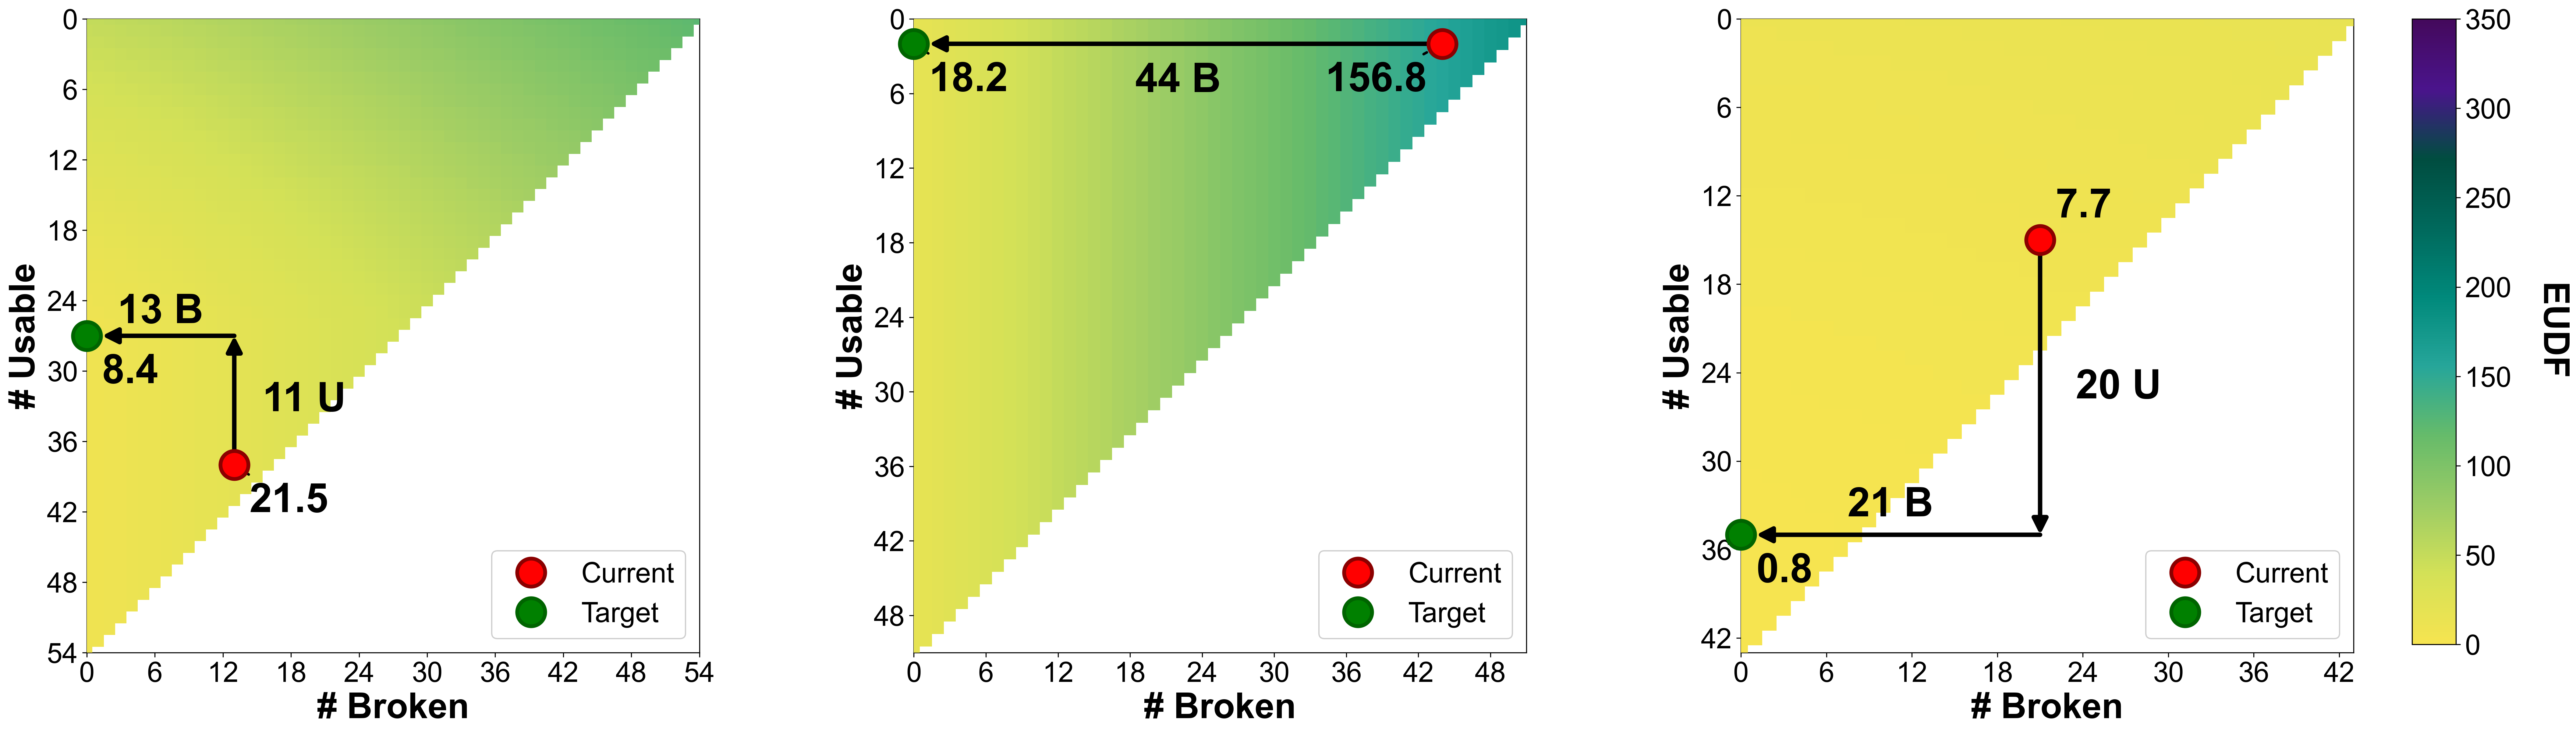
\includegraphics[width=.88\linewidth]{figures/heatmap-of-eudf.png}
    \end{minipage}

\end{block}

        \end{minipage}
    };
    
    % Section 5 - Column 3, Row 1
    \node[anchor=north east, inner sep=0] at ([xshift=-\contentmargin, yshift=-\headerheight-\rowgap]current page.north east) {
        \begin{minipage}[t][\colthreerowoneheight][t]{\colwidth}
            \setlength{\textwidth}{\colwidth}\setlength{\linewidth}{\colwidth}
            % Section 5: Numerical Studies
\begin{block}{\fontsize{46}{54}\selectfont 5. Numerical Studies}

{\fontsize{40}{48}\selectfont \textbf{A) Solver Comparison (HGS vs Gurobi)}}

\vspace{0.3cm}
\noindent
\begin{minipage}[t]{0.26\linewidth}
    \vspace{0pt}
    {\fontsize{34}{42}\selectfont \textbf{Small Instances}}\\[0.15cm]
    {\fontsize{28}{34}\selectfont $|S|\le 15$, $|K|{=}|R|{=}1$}\\[0.1cm]
    {\fontsize{28}{34}\selectfont All solved to \textbf{optimality}.}
    
    \vspace{0.3cm}
    {\fontsize{28}{34}\selectfont CPU times (s): Gurobi vs HGS}
    
    \vspace{0.25cm}
    \renewcommand{\arraystretch}{1.25}
    {\fontsize{26}{32}\selectfont
    \begin{tabular*}{\linewidth}{@{\extracolsep{\fill}}c r r@{}}
        \toprule
        \multicolumn{3}{c}{\textbf{$|S|=6$}} \\
        \midrule
        inst. & Gurobi & HGS \\
        \midrule
        1 & 13.41 & 6.29 \\
        2 & 13.85 & 5.75 \\
        3 & 66.97 & 6.22 \\
        4 & 2.29  & 3.63 \\
        5 & 22.29 & 4.84 \\
        \bottomrule
    \end{tabular*}}
    
    \vspace{0.2cm}
    {\fontsize{26}{32}\selectfont
    \begin{tabular*}{\linewidth}{@{\extracolsep{\fill}}c r r@{}}
        \toprule
        \multicolumn{3}{c}{\textbf{$|S|=10$}} \\
        \midrule
        inst. & Gurobi & HGS \\
        \midrule
        1 & 928.50   & 3.87 \\
        2 & 1409.89  & 5.27 \\
        3 & 13768.72 & 3.02 \\
        4 & 2404.03  & 5.16 \\
        5 & 4172.75  & 4.17 \\
        \bottomrule
    \end{tabular*}}
    
    \vspace{0.2cm}
    {\fontsize{26}{32}\selectfont
    \begin{tabular*}{\linewidth}{@{\extracolsep{\fill}}c r r@{}}
        \toprule
        \multicolumn{3}{c}{\textbf{$|S|=15$}} \\
        \midrule
        inst. & Gurobi & HGS \\
        \midrule
        1 & 2602.24 & 7.80 \\
        2 & 4209.67 & 4.89 \\
        3 & 6283.58 & 4.72 \\
        4 & 3374.38 & 5.32 \\
        5 & 2371.40 & 5.08 \\
        \bottomrule
    \end{tabular*}}
\end{minipage}%
\hspace{0.01\linewidth}%
\vrule width 1.5pt%
\hspace{0.01\linewidth}%
\begin{minipage}[t]{0.70\linewidth}
    \vspace{0pt}
    {\fontsize{34}{42}\selectfont \textbf{Large Instances (Scalability):} $|S|=60$--500, $K\in\{1,2\}$, $R\in\{1,2\}$.}
    
    \vspace{0.25cm}
    \renewcommand{\arraystretch}{1.25}
    \setlength{\tabcolsep}{10pt}
    {\fontsize{26}{32}\selectfont
    \begin{tabular*}{\linewidth}{@{\extracolsep{\fill}}c rrr rrr rrr rrr rr@{}}
        \toprule
        & \multicolumn{3}{c}{\boldmath$K{=}1, R{=}1$} & \multicolumn{3}{c}{\boldmath$K{=}1, R{=}2$} & \multicolumn{3}{c}{\boldmath$K{=}2, R{=}1$} & \multicolumn{3}{c}{\boldmath$K{=}2, R{=}2$} & \multicolumn{2}{c}{\textbf{CPU (s)}} \\
        \cmidrule(lr){2-4} \cmidrule(lr){5-7} \cmidrule(lr){8-10} \cmidrule(lr){11-13} \cmidrule(lr){14-15}
        $|S|$ & $O_{\text{H}}$ & $O_{\text{G}}$ & Gap & $O_{\text{H}}$ & $O_{\text{G}}$ & Gap & $O_{\text{H}}$ & $O_{\text{G}}$ & Gap & $O_{\text{H}}$ & $O_{\text{G}}$ & Gap & Grb & HGS \\
        \midrule
        \multicolumn{15}{c}{\textbf{$T=2$ h}} \\
        \midrule
        60  & 2581 & 2605 & 0.9 & 2494 & 2533 & 1.6 & 2401 & 3582 & 33.0 & 2325 & 3518 & 33.9 & 7200 & 6--11 \\
        90  & 4038 & 4511 & 10.5 & 3942 & 4159 & 5.2 & 3862 & 4511 & 14.4 & 3769 & 4489 & 16.0 & 7200 & 9--13 \\
        120 & 4303 & 5114 & 15.9 & 4238 & 5104 & 17.0 & 4168 & 5114 & 18.5 & 4097 & 5104 & 19.7 & 7200 & 9--16 \\
        200 & 7821 & 8657 & 9.7 & 7720 & 8657 & 10.8 & 7642 & 8657 & 11.7 & 7561 & 8657 & 12.7 & 7200 & 12--24 \\
        300 & 11169 & 11717 & 4.7 & 11058 & 11717 & 5.6 & 10989 & 11717 & 6.2 & 10888 & 11717 & 7.1 & 7200 & 17--34 \\
        400 & 14281 & 15069 & 5.2 & 14179 & 15061 & 5.9 & 14169 & 15069 & 6.0 & 14059 & 15061 & 6.7 & 7200 & 25--44 \\
        500 & 18962 & 19794 & 4.2 & 18793 & 19785 & 5.0 & 18752 & 19794$^\dagger$ & 5.3 & 18613 & 19785$^\dagger$ & 5.9 & 7200 & 27--51 \\
        \midrule
        \multicolumn{15}{c}{\textbf{$T=3$ h}} \\
        \midrule
        60  & 2433 & 3554 & 31.5 & 2365 & 3507 & 32.6 & 2265 & 3582 & 36.8 & 2214 & 3507 & 36.9 & 7200 & 10--14 \\
        90  & 3903 & 4504 & 13.3 & 3779 & 4481 & 15.7 & 3705 & 4504 & 17.7 & 3607 & 4481 & 19.5 & 7200 & 10--20 \\
        120 & 4203 & 5114 & 17.8 & 4107 & 5104 & 19.5 & 4024 & 5114 & 21.3 & 3952 & 5104 & 22.6 & 7200 & 9--18 \\
        200 & 7695 & 8657 & 11.1 & 7575 & 8657 & 12.5 & 7471 & 8657 & 13.7 & 7394 & 8657 & 14.6 & 7200 & 14--28 \\
        300 & 11024 & 11716 & 5.9 & 10901 & 11716 & 7.0 & 10830 & 11716 & 7.6 & 10693 & 11716 & 8.7 & 7200 & 18--44 \\
        400 & 14138 & 15069 & 6.2 & 14010 & 15061 & 7.0 & 13969 & 15069$^\dagger$ & 7.3 & 13852 & 15061$^\dagger$ & 8.0 & 7200 & 22--56 \\
        500 & 18818 & 19794 & 4.9 & 18596 & 19785$^\dagger$ & 6.0 & 18572 & 19794$^\dagger$ & 6.2 & 18407 & 19785$^\dagger$ & 7.0 & 7200 & 22--62 \\
        \bottomrule
    \end{tabular*}}
    
    \vspace{0.3cm}
    % Two-column layout for Setup/Symbols and Summary - equal height boxes
    \noindent
    \begin{minipage}[t]{0.485\linewidth}
        \vspace{0pt}
        \colorbox{DarkSlate!8}{\parbox[t][8.5cm][t]{0.96\linewidth}{
            \vspace{0.2cm}
            {\fontsize{28}{34}\selectfont \textbf{Setup \& Notation}}
            
            \vspace{0.2cm}
            {\fontsize{24}{30}\selectfont
            $\bullet$ $CPU^{\text{max}}=7200$ s time limit, 20 runs per instance\\[0.15cm]
            $\bullet$ Repositioning time budget $T\in\{2,3\}$ hours\\[0.15cm]
            $\bullet$ $O_{\text{H}}$: HGS objective (avg. over 20 runs)\\[0.15cm]
            $\bullet$ $O_{\text{G}}$: Gurobi upper bound\\[0.15cm]
            $\bullet$ Gap $= 100\times(O_{\text{G}}-O_{\text{H}})/O_{\text{G}}$\\
            $\bullet$ \colorbox{red!15}{$^\dagger$ Gurobi ran out of memory (64GB)}
            }
        }}
    \end{minipage}%
    \hspace{0.02\linewidth}%
    \begin{minipage}[t]{0.495\linewidth}
        \vspace{0pt}
        \colorbox{AccentGold!22}{\parbox[t][8.5cm][t]{0.98\linewidth}{
            \vspace{0.2cm}
            {\fontsize{28}{34}\selectfont \textbf{Key Findings}}
            
            \vspace{0.2cm}
            {\fontsize{24}{30}\selectfont
            \textbf{Small instances} ($|S|\le 15$):\\[0.15cm]
            \ding{51} HGS matches \textbf{optimal} solutions in all cases\\[0.15cm]
            \ding{51} HGS: \textbf{3--8 seconds} vs Gurobi: \textbf{minutes--hours}\\[0.3cm]
            \textbf{Large instances} ($|S|=60$--500):\\[0.15cm] 
            \ding{51} HGS improves Gurobi UB by up to \textbf{33.9\%} within \textbf{6--62 seconds}\\[0.15cm]
            \ding{51} Gurobi hits 2h time limit to find a worse solution or crashes (64GB)
            }
        }}
    \end{minipage}
\end{minipage}

\vspace{0.4cm}
\hrule
\vspace{0.4cm}

{\fontsize{40}{48}\selectfont \textbf{B) When Are On-Site Repairers Cost-Effective?}}

\vspace{0.3cm}
\noindent
\begin{minipage}[t][22cm][t]{0.52\linewidth}
    \vspace{0pt}
    {\fontsize{34}{42}\selectfont Cost-effectiveness $\nu$ vs repair time (selected $\ell$ values):}
    
    \vspace{0.3cm}
    \centering
    \begin{tabular}{@{}cc@{}}
        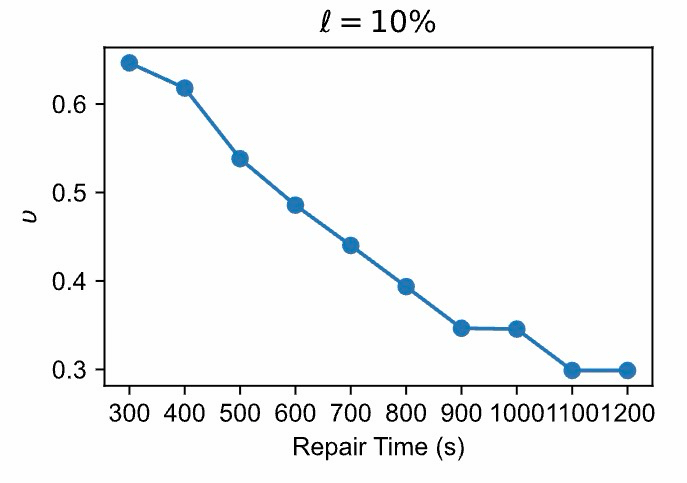
\includegraphics[width=0.48\linewidth]{figures/cost_effectiveness_l10.png} &
        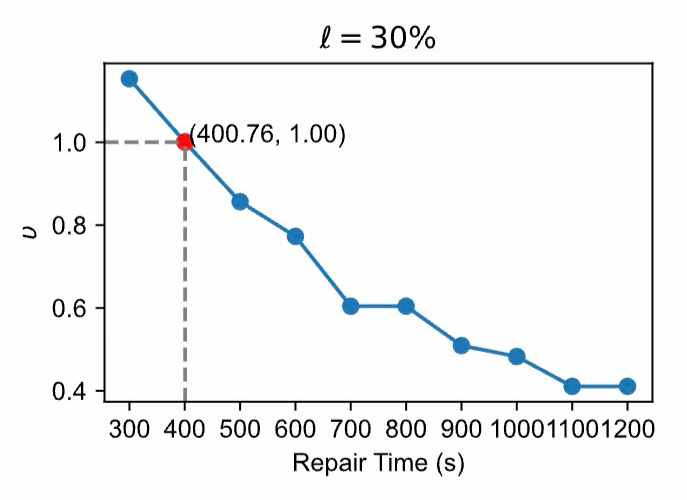
\includegraphics[width=0.48\linewidth]{figures/cost_effectiveness_l30.png} \\[0.3cm]
        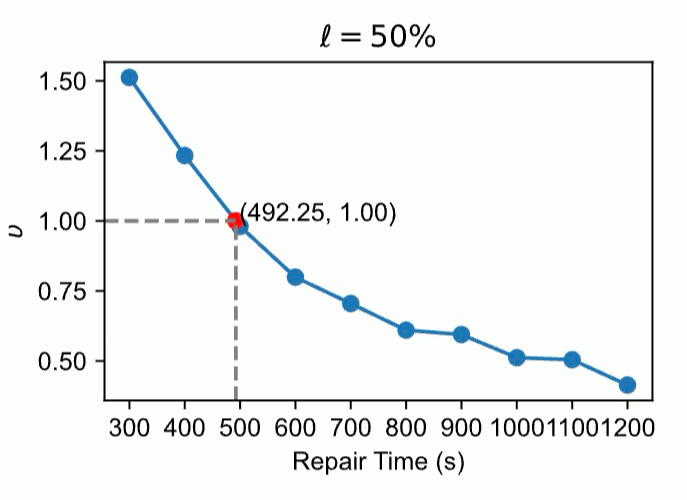
\includegraphics[width=0.48\linewidth]{figures/cost_effectiveness_l50.png} &
        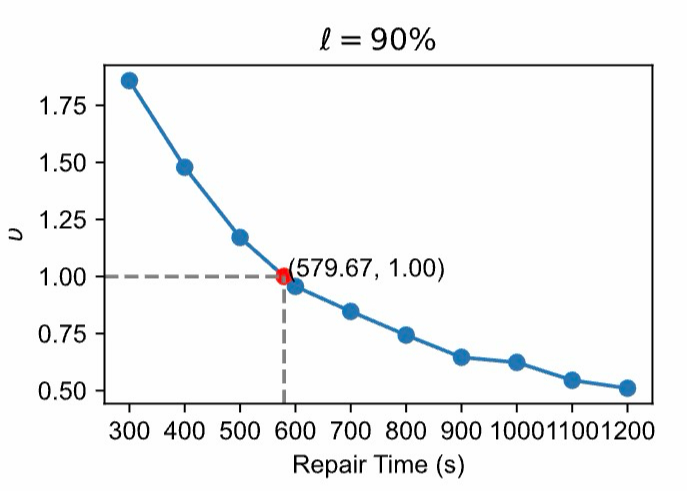
\includegraphics[width=0.48\linewidth]{figures/cost_effectiveness_l90.png} \\
    \end{tabular}
\end{minipage}%
\hspace{0.02\linewidth}%
\begin{minipage}[t][22cm][s]{0.44\linewidth}
    % Match the title line height from left column
    \vspace{1.8cm}
    
    \colorbox{HKUGreen!10}{\parbox{0.96\linewidth}{
        \vspace{0.3cm}
        {\fontsize{40}{48}\selectfont \textbf{Cost-Effectiveness Indicator}}
        
        \vspace{0.55cm}
        \begin{center}
        {\fontsize{48}{58}\selectfont $\displaystyle \nu = \frac{c^p \cdot \Delta F}{\varpi \cdot T/3600}$}
        \end{center}
        
        \vspace{0.55cm}
        {\fontsize{40}{48}\selectfont
        $\bullet$ $\Delta F$: dissatisfaction reduction\\[0.5cm]
        $\bullet$ $c^p$: penalty cost per unit dissatisfaction\\[0.5cm]
        $\bullet$ $\varpi$: repairer hourly wage\\[0.5cm]
        $\bullet$ $\nu$ measures \textbf{benefit per wage}
        }
        \vspace{0.3cm}
    }}
    
    \vspace{0.8cm}
    
    \colorbox{AccentGold!20}{\parbox{0.96\linewidth}{
        \vspace{0.3cm}
        {\fontsize{40}{48}\selectfont \textbf{Key Findings}}
        
        \vspace{0.35cm}
        {\fontsize{40}{48}\selectfont
        \ding{51} \textbf{Low $\ell$ ($\le 20\%$):} repairers \textbf{never} pay off\\[0.15cm]
        \hspace{0.6cm}{\fontsize{40}{48}\selectfont (curves always below $\nu=1$)}\\[0.65cm]
        \ding{51} \textbf{Higher $\ell$} $\Rightarrow$ larger tolerance for\\[0.15cm]
        \hspace{0.6cm}{\fontsize{40}{48}\selectfont slower repairs (\textbf{401--600 s})}\\[0.65cm]
        \ding{51} \textbf{Practical rule:}\\[0.55cm]
        \hspace{0.6cm}{\fontsize{40}{48}\selectfont Deploy repairers when $\ell \ge 30\%$}\\[0.15cm]
        \hspace{0.6cm}{\fontsize{40}{48}\selectfont and repair time $\lesssim 7$--10 min}
        }
        \vspace{0.3cm}
    }}
    
    \vspace{0pt}
\end{minipage}

\end{block}

        \end{minipage}
    };
    
    % ---------------------------------------------------------
    % ROW 2: Sections 2, 4, 6 (bottom row)
    % ---------------------------------------------------------
    
    % Section 2 - Column 1, Row 2
    \node[anchor=north west, inner sep=0] at ([xshift=\contentmargin, yshift=-\headerheight-\rowgap-\rowoneheight-\rowgap]current page.north west) {
        \begin{minipage}[t][\rowtwoheight][t]{\colwidth}
            \setlength{\textwidth}{\colwidth}\setlength{\linewidth}{\colwidth}
            % Section 2: Problem Description & Model
% Compact contributions, expand mathematical model
\begin{block}{\fontsize{46}{54}\selectfont 2. Problem Description \& Model}
    
    {\fontsize{40}{48}\selectfont \textbf{Problem Illustration:}}
    
    \vspace{0.4cm}
    \noindent
    % Two figures side by side: Spatial network | Temporal process
    \begin{minipage}[t]{0.48\linewidth}
        \vspace{0pt}
        \centering
        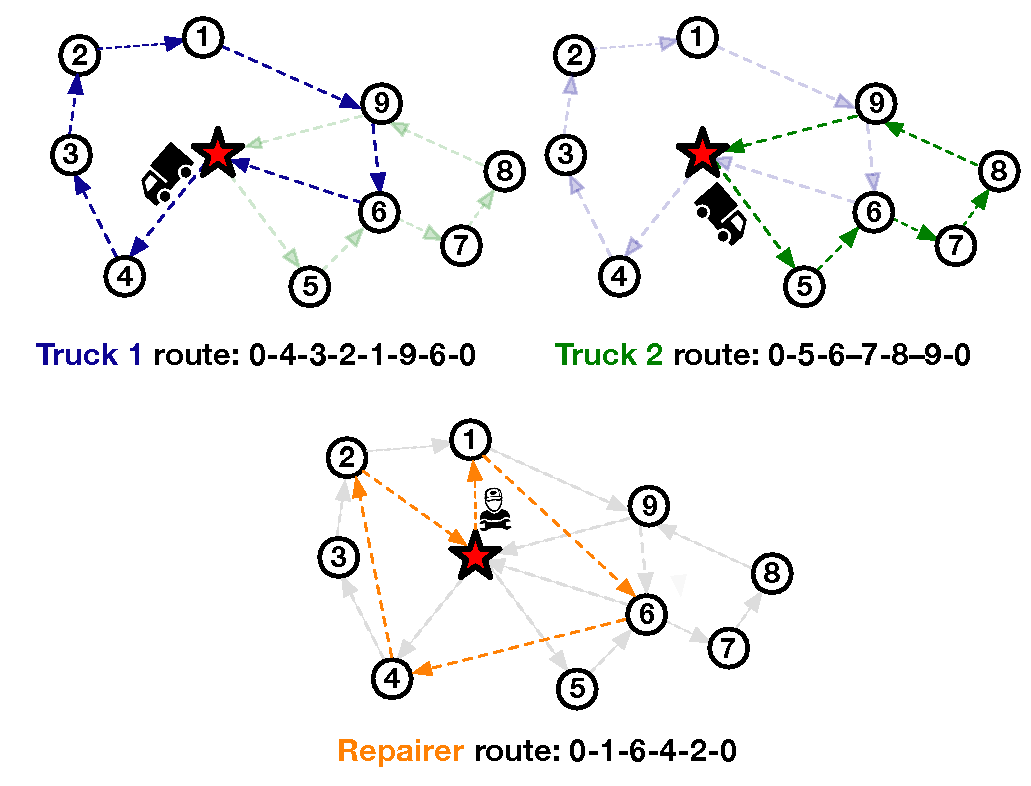
\includegraphics[width=\linewidth,height=26cm,keepaspectratio]{figures/add_repairer.pdf}
        
        \vspace{0.3cm}
        {\fontsize{34}{40}\selectfont \textbf{(a)} Spatial: Network with trucks \& repairers}
    \end{minipage}%
    \hfill
    \begin{minipage}[t]{0.48\linewidth}
        \vspace{0pt}
        \centering
        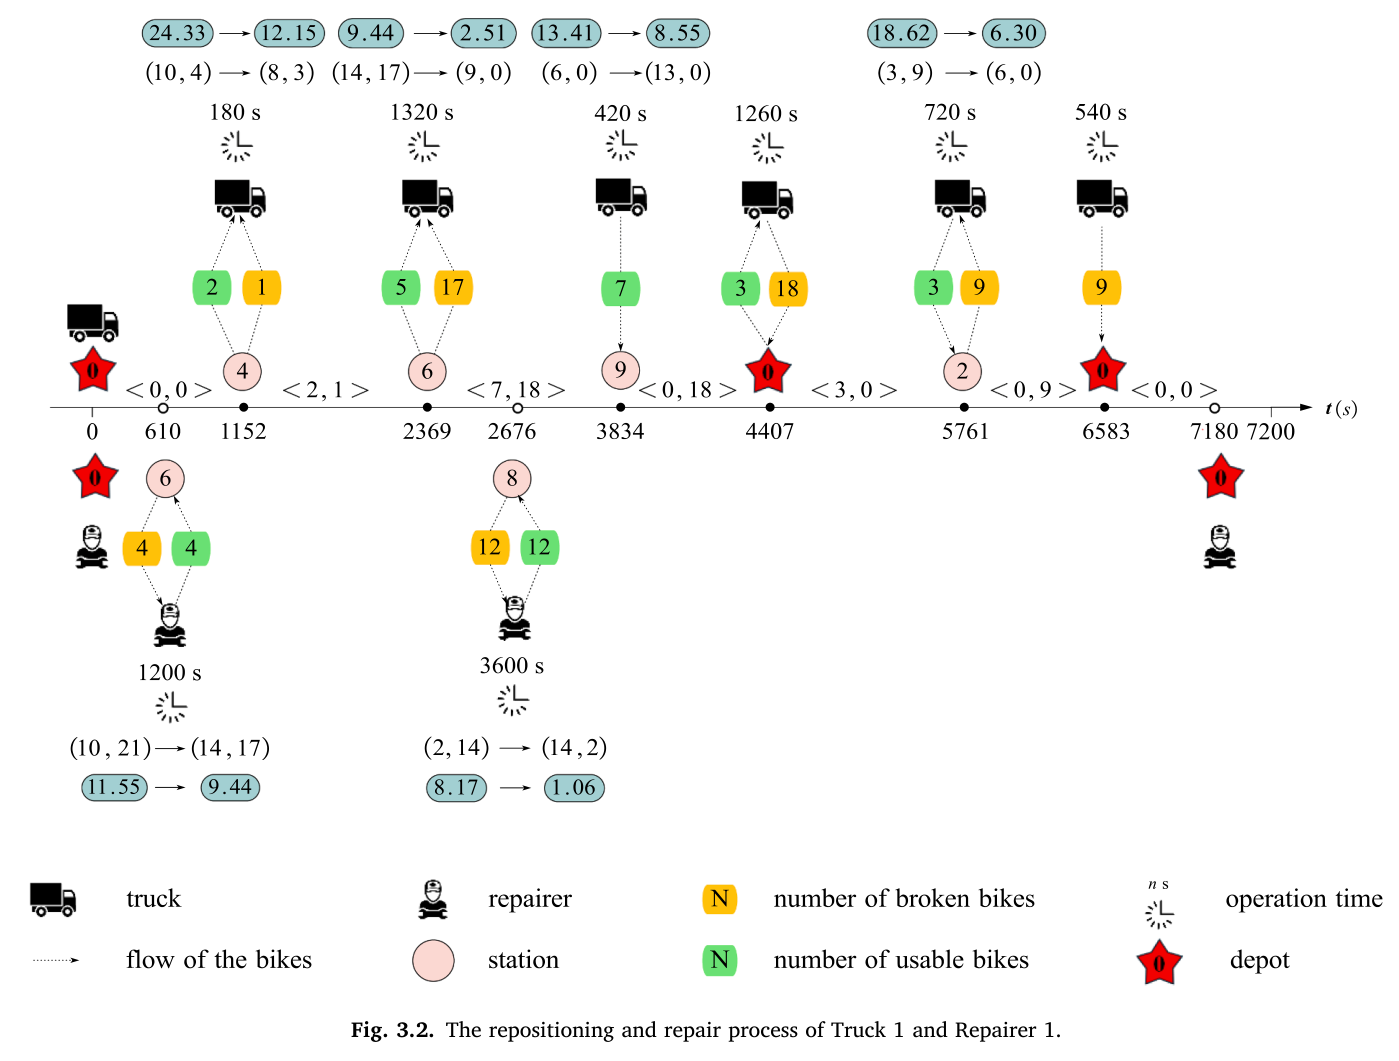
\includegraphics[width=\linewidth,height=26cm,keepaspectratio]{figures/fig_3_2_temporal_illustration.png}
        
        \vspace{0.3cm}
        {\fontsize{34}{40}\selectfont \textbf{(b)} Temporal: Repositioning \& repair process}
    \end{minipage}
    
    \vspace{0.6cm}
    \hrule
    \vspace{0.5cm}
    
    {\fontsize{40}{48}\selectfont \textbf{Mathematical Model (MILP):}}
    
    \vspace{0.4cm}
    {\fontsize{36}{44}\selectfont
    \begin{tabular}{@{}p{0.30\linewidth}p{0.32\linewidth}p{0.34\linewidth}@{}}
        \textbf{Objective:} & \textbf{Key Decision Variables:} & \textbf{Key Constraints:} \\[0.4cm]
        \quad $\bullet$ User dissat. $F_i(\#usable, \#broken)$ & \quad $\bullet$ Routings of trucks \& repairers & \quad $\bullet$ Time budget $T$ for all vehicles \\[0.3cm]
        \quad $\bullet$ CO$_2$ emissions from trucks & \quad $\bullet$ Usable bikes load/unload qty & \quad $\bullet$ Truck capacity (usable + broken) \\[0.3cm]
        & \quad $\bullet$ Broken bikes load/unload/repair qty & \quad $\bullet$ Station inventory balance \\[0.3cm]
        & & \quad $\bullet$ Flow conservation \\
    \end{tabular}}
    
    \vspace{0.6cm}
    \hrule
    \vspace{0.5cm}
    
    {\fontsize{40}{48}\selectfont \textbf{Our Contributions:}}
    
    \vspace{0.5cm}
    \noindent
    \colorbox{HKUGreen!20}{\parbox{0.23\linewidth}{\centering
        \vspace{0.3cm}
        {\fontsize{34}{40}\selectfont \textbf{Novel Problem}}\\[0.25cm]
        {\fontsize{30}{36}\selectfont First to integrate\\on-site repairs}
        \vspace{0.3cm}
    }}%
    \hfill
    \colorbox{AccentGold!25}{\parbox{0.23\linewidth}{\centering
        \vspace{0.3cm}
        {\fontsize{34}{40}\selectfont \textbf{MILP Model}}\\[0.25cm]
        {\fontsize{30}{36}\selectfont Time-indexed\\formulation}
        \vspace{0.3cm}
    }}%
    \hfill
    \colorbox{HKUGreen!20}{\parbox{0.23\linewidth}{\centering
        \vspace{0.3cm}
        {\fontsize{34}{40}\selectfont \textbf{HGS-ADC+SBC}}\\[0.25cm]
        {\fontsize{30}{36}\selectfont Scalable\\algorithm}
        \vspace{0.3cm}
    }}%
    \hfill
    \colorbox{AccentGold!25}{\parbox{0.23\linewidth}{\centering
        \vspace{0.3cm}
        {\fontsize{34}{40}\selectfont \textbf{Insights}}\\[0.25cm]
        {\fontsize{30}{36}\selectfont Cost-effectiveness\\analysis}
        \vspace{0.3cm}
    }}

\end{block}

        \end{minipage}
    };
    
    % Section 4 - Column 2, Row 2
    \node[anchor=north, inner sep=0] at ([yshift=-\headerheight-\rowgap-\rowoneheight-\rowgap]current page.north) {
        \begin{minipage}[t][\rowtwoheight][t]{\colwidth}
            \setlength{\textwidth}{\colwidth}\setlength{\linewidth}{\colwidth}
            % Section 4: Key Innovation - SBC & BCRF
\begin{block}{\fontsize{46}{54}\selectfont 4. Key Innovation: Station-Budget-Constrained (SBC) Allocation}

% =========================================================
% A. Before vs After (what goes wrong, what SBC fixes)
% =========================================================
\noindent
\begin{minipage}[t]{0.485\linewidth}
    \centering
    {\fontsize{38}{46}\selectfont \textbf{\textcolor{AlertRed}{Greedy (No Cap)}}}

    \vspace{0.3cm}
    {\fontsize{30}{36}\selectfont Service time share across stations}

    \vspace{0.3cm}
    \begin{tikzpicture}[x=2.6cm,y=0.11cm,transform shape]
        % Fix bounding box so the "Greedy" and "SBC" mini-charts have identical height
        \path[use as bounding box] (-0.8,-15) rectangle (5.6,95);
        % Greedy with route Depot->3->1->2: Stn3=80%, Stn1=15%, Stn2=5%
        \fill[AlertRed!55] (0,0) rectangle (1.1,15);
        \fill[AlertRed!35] (1.7,0) rectangle (2.8,5);
        \fill[AlertRed!80] (3.4,0) rectangle (4.5,80);

        \node[font=\fontsize{28}{34}\selectfont\bfseries,text=AlertRed,anchor=south] at (0.55,15) {15\%};
        \node[font=\fontsize{28}{34}\selectfont\bfseries,text=AlertRed,anchor=south] at (2.25,5) {5\%};
        \node[font=\fontsize{28}{34}\selectfont\bfseries,text=AlertRed,anchor=south] at (3.95,80) {80\%};

        \node[font=\fontsize{26}{32}\selectfont] at (0.55,-10) {Stn1};
        \node[font=\fontsize{26}{32}\selectfont] at (2.25,-10) {Stn2};
        \node[font=\fontsize{26}{32}\selectfont] at (3.95,-10) {Stn3};

        \draw[DarkSlate!55,line width=2pt] (-0.3,0) -- (4.6,0);
        
        % Annotation for Station 2 - high BCRF but lowest share (left side)
        \node[
            anchor=east,
            font=\fontsize{26}{32}\selectfont,
            text=DarkSlate,
            align=left,
            fill=white,
            draw=DarkSlate!60,
            line width=1.5pt,
            rounded corners=4pt,
            inner sep=7pt
        ] (ann2) at (2.9,42) {High BCRF\\but only 5\% service \\ time allocated!};
        \draw[-{Stealth[length=3mm,width=2.5mm]},line width=1.5pt,DarkSlate!70] 
            (ann2.south) -- (2.25,10);
        
        % Annotation for Station 3 - low BCRF but highest share (RIGHT side)
        \node[
            anchor=west,
            font=\fontsize{26}{32}\selectfont,
            text=AlertRed!80!black,
            align=left,
            fill=AlertRed!10,
            draw=AlertRed!70,
            line width=1.5pt,
            rounded corners=4pt,
            inner sep=7pt
        ] (ann3) at (5.65,85) {Low BCRF\\but 80\% service \\ time allocated!};
        \draw[-{Stealth[length=3mm,width=2.5mm]},line width=1.5pt,AlertRed!70] 
            (ann3.west) -- (4.45,82);
    \end{tikzpicture}

    \vspace{0.3cm}
    \textcolor{AlertRed}{\fontsize{28}{34}\selectfont \ding{55} Early stations consume the remaining service time}
\end{minipage}%
\hfill
\begin{minipage}[t]{0.485\linewidth}
    \centering
    {\fontsize{38}{46}\selectfont \textbf{\textcolor{HKUGreen}{SBC (With Cap)}}}

    \vspace{0.3cm}
    {\fontsize{30}{36}\selectfont Service time share across stations}

    \vspace{0.3cm}
    \begin{tikzpicture}[x=2.6cm,y=0.11cm,transform shape]
        % Fix bounding box so the "Greedy" and "SBC" mini-charts have identical height
        \path[use as bounding box] (-0.4,-15) rectangle (4.8,95);
        % SBC based on BCRF: Stn1=14%, Stn2=82%, Stn3=4%
        \fill[HKUGreen!55] (0,0) rectangle (1.1,14);
        \fill[HKUGreen!70] (1.7,0) rectangle (2.8,82);
        \fill[HKUGreen!45] (3.4,0) rectangle (4.5,4);

        \node[font=\fontsize{28}{34}\selectfont\bfseries,text=HKUGreen!80!black,anchor=south] at (0.55,14) {14\%};
        \node[font=\fontsize{28}{34}\selectfont\bfseries,text=HKUGreen!80!black,anchor=south] at (2.25,82) {82\%};
        \node[font=\fontsize{28}{34}\selectfont\bfseries,text=HKUGreen!80!black,anchor=south] at (3.95,4) {4\%};

        \node[font=\fontsize{26}{32}\selectfont] at (0.55,-10) {Stn1};
        \node[font=\fontsize{26}{32}\selectfont] at (2.25,-10) {Stn2};
        \node[font=\fontsize{26}{32}\selectfont] at (3.95,-10) {Stn3};

        \draw[DarkSlate!55,line width=2pt] (-0.3,0) -- (4.6,0);
        
        % Annotation for Station 2 - highest BCRF
        \node[
            anchor=west,
            font=\fontsize{26}{32}\selectfont,
            text=AccentGold!90!black,
            align=left,
            fill=AccentGold!15,
            draw=AccentGold,
            line width=1.5pt,
            rounded corners=5pt,
            inner sep=7pt
        ] (annotation) at (6.0,108) {Highest BCRF\\$\Rightarrow$ worth investing};
        
        % Arrow from annotation to bar
        \draw[-{Stealth[length=3mm,width=2.5mm]},line width=1.5pt,AccentGold!80!black] 
            (annotation.south west) -- (2.65,85);
    \end{tikzpicture}

    \vspace{0.3cm}
    \textcolor{HKUGreen}{\fontsize{28}{34}\selectfont \ding{51} All stations are guaranteed nonzero service}
\end{minipage}

\vspace{0.5cm}

\colorbox{AccentGold!18}{\parbox{0.98\linewidth}{
    \vspace{0.15cm}
    {\fontsize{32}{40}\selectfont \textbf{Key idea:} Use \textbf{BCRF} to pre-allocate \textbf{station-level service-time budgets} and enforce them as caps.}
    \vspace{0.15cm}
}}

\vspace{0.6cm}

% =========================================================
% B. Step 1 & Step 2 (BCRF + budget allocation)
% =========================================================
\noindent
\begin{minipage}[t]{0.54\linewidth}
    {\fontsize{36}{44}\selectfont \textbf{Step 1: Compute Benefit--Cost Ratio Function}}

    \vspace{0.3cm}
    \colorbox{HKUGreen!10}{\parbox{0.97\linewidth}{\centering
        \vspace{0.4cm}
        {\fontsize{38}{46}\selectfont
        $\displaystyle
        BCRF_s^{\text{t}}(p,b)=\frac{F_s(p,b)-F_s(q,0)}{t^{load}\cdot\bigl(|q-p|+b\bigr)}
        $}
        \vspace{0.4cm}
    }}

    \vspace{0.3cm}
    {\fontsize{28}{34}\selectfont
    \begin{tabular}{@{}p{0.47\linewidth}@{\hspace{0.35cm}}p{0.47\linewidth}@{}}
        \textbf{$F_s(\cdot)$}: dissat. at station $s$ &
        \textbf{$t^{load}$}: per-bike handling time \\[0.15cm]
        \textbf{$q$}: target usable bike inventory &
        \textbf{$p$}: current usable bike inventory \\[0.15cm]
        \textbf{$b$}: broken bikes handled & \\
    \end{tabular}
    }
\end{minipage}%
\hfill
\begin{minipage}[t]{0.44\linewidth}
    {\fontsize{36}{44}\selectfont \textbf{Step 2: Allocate station budgets}}

    \vspace{0.3cm}
    \colorbox{HKUGreen!10}{\parbox{0.97\linewidth}{\centering
        \vspace{0.4cm}
        {\fontsize{38}{46}\selectfont
        $\displaystyle
        B_s = T^\text{svc}\cdot\frac{BCRF_s}{\sum_{j\in \mathcal{R}} BCRF_j}
        $}
        \vspace{0.4cm}
    }}

    \vspace{0.3cm}
    {\fontsize{28}{34}\selectfont
    \begin{tabular}{@{}p{0.5\linewidth}@{\hspace{0.35cm}}p{0.47\linewidth}@{}}
        \textbf{$T^\text{svc}$}: total service time budget &
        \textbf{$\mathcal{R}$}: visited stations \\
    \end{tabular}

    \vspace{0.15cm}
    Higher BCRF $\Rightarrow$ larger budget.
    }
\end{minipage}

\vspace{0.4cm}

\begin{center}
    \begin{tikzpicture}[scale=1.0,transform shape]
        % Total budget box - width 75
        \fill[DarkSlate!12] (0,0) rectangle (75,2.4);
        \draw[line width=2.2pt,DarkSlate] (0,0) rectangle (75,2.4);
        \node[font=\fontsize{34}{42}\selectfont\bfseries] at (37.5,1.2) {Total Station Service-Time Budget $T^\text{svc}$ = 100 min};

        % Station boxes — widths proportional to BCRF shares (0.14, 0.82, 0.04)
        % Based on BCRF: Stn1=0.55, Stn2=3.15, Stn3=0.17 → normalized: 14%, 82%, 4%
        % Total width 75, gaps ~1.5 each (total ~3.0), box space = ~72.0
        % Stn 1: 0.14 × 72 = 10, Stn 2: 0.82 × 72 = 59, Stn 3: 0.04 × 72 = 3
        % Stn 1: 0 to 10, Stn 2: 11.5 to 70.5, Stn 3: 72 to 75
        \fill[HKUGreen!45] (0,-6.2) rectangle (10,-3.0);
        \draw[line width=2.2pt,HKUGreen!80!black] (0,-6.2) rectangle (10,-3.0);
        \draw[line width=5pt,AlertRed] (0,-3.0) -- (10,-3.0);
        \node[font=\fontsize{28}{34}\selectfont\bfseries,align=center] at (5,-4.6) {Stn 1: 14 min};
        \node[font=\fontsize{24}{30}\selectfont,text=HKUGreen!70!black,anchor=north] at (5,-6.5) {BCRF = 0.14};

        \fill[HKUGreen!65] (11.5,-6.2) rectangle (70.5,-3.0);
        \draw[line width=2.2pt,HKUGreen!80!black] (11.5,-6.2) rectangle (70.5,-3.0);
        \draw[line width=5pt,AlertRed] (11.5,-3.0) -- (70.5,-3.0);
        \node[font=\fontsize{30}{36}\selectfont\bfseries,align=center] at (41,-4.6) {Stn 2: 82 min};
        \node[font=\fontsize{26}{32}\selectfont,text=HKUGreen!70!black,anchor=north] at (41,-6.5) {BCRF = 0.82};

        \fill[HKUGreen!35] (72,-6.2) rectangle (75,-3.0);
        \draw[line width=2.2pt,HKUGreen!80!black] (72,-6.2) rectangle (75,-3.0);
        \draw[line width=5pt,AlertRed] (72,-3.0) -- (75,-3.0);
        \node[font=\fontsize{22}{28}\selectfont\bfseries,align=center] at (73.5,-4.3) {Stn 3:\\ 4 min};
        \node[font=\fontsize{20}{26}\selectfont,text=HKUGreen!70!black,anchor=north] at (73.5,-6.5) {BCRF = 0.04};

        % Arrows — straight down from parent box to each station box (at box centers)
        \draw[-{Stealth},line width=4pt,AccentGold] (5,-0.1) -- (5,-3.0);
        \draw[-{Stealth},line width=4pt,AccentGold] (41,-0.1) -- (41,-3.0);
        \draw[-{Stealth},line width=4pt,AccentGold] (73.5,-0.1) -- (73.5,-3.0);
        
        % Central label between parent and station boxes
        \node[font=\fontsize{28}{34}\selectfont\bfseries,text=AccentGold,fill=white,inner sep=5pt] at (37.5,-1.55) {Allocate proportional to BCRF};
        
        % Red cap labels positioned above the red lines
        \node[font=\fontsize{22}{28}\selectfont\bfseries,text=AlertRed] at (5,-3.35) {cap};
        \node[font=\fontsize{24}{30}\selectfont\bfseries,text=AlertRed] at (41,-3.4) {cap};
        \node[font=\fontsize{18}{24}\selectfont\bfseries,text=AlertRed] at (73.5,-3.32) {cap};
    \end{tikzpicture}
\end{center}

\vspace{0.4cm}

% =========================================================
% C. Step 3 (cap changes the quantity assignment rule)
% =========================================================
{\fontsize{36}{44}\selectfont \textbf{Step 3: Quantity assignment (what changes)}}

\vspace{0.25cm}
{\fontsize{30}{36}\selectfont Actions must satisfy $t^\text{load}\cdot\bigl(|q-p|+b\bigr)\le \text{cap}$.}

\vspace{0.4cm}
\noindent
\begin{minipage}[t]{0.485\linewidth}
    \colorbox{AlertRed!8}{\parbox{0.97\linewidth}{\centering
        \vspace{0.35cm}
        {\fontsize{30}{36}\selectfont \textbf{Greedy:} cap = \colorbox{AlertRed!25}{\textbf{remaining time budget}}}

        \vspace{0.25cm}
        {\fontsize{28}{34}\selectfont $\Rightarrow$ early stations can still monopolize time.}
        \vspace{0.35cm}
    }}
\end{minipage}%
\hfill
\begin{minipage}[t]{0.485\linewidth}
    \colorbox{HKUGreen!8}{\parbox{0.97\linewidth}{\centering
        \vspace{0.35cm}
        {\fontsize{30}{36}\selectfont \textbf{SBC:} cap = \colorbox{HKUGreen!25}{\textbf{station budget $B_s$ (+carryover)}}}

        \vspace{0.25cm}
        {\fontsize{28}{34}\selectfont $\Rightarrow$ each station respects its budget cap.}
        \vspace{0.35cm}
    }}
\end{minipage}

\vspace{0.5cm}
\colorbox{AccentGold!18}{\parbox{0.98\linewidth}{
    \vspace{0.15cm}
    {\fontsize{32}{40}\selectfont SBC makes greedy quantity assignment \textbf{fair} by adding a \textbf{station-level time cap} driven by BCRF.}
    \vspace{0.15cm}
}}

\end{block}

        \end{minipage}
    };
    
    % Section 6 - Column 3, Row 2
    \node[anchor=north east, inner sep=0] at ([xshift=-\contentmargin, yshift=-\headerheight-\rowgap-\colthreerowoneheight-\rowgap]current page.north east) {
        \begin{minipage}[t][\colthreerowtwoheight][t]{\colwidth}
            \setlength{\textwidth}{\colwidth}\setlength{\linewidth}{\colwidth}
            % Section 6: Conclusions & Future Work
\begin{block}{\fontsize{46}{54}\selectfont 6. Conclusions \& Future Work}
    \vspace{0.5cm}
    % Two columns: Text left, QR codes right
    \begin{minipage}[t]{0.54\linewidth}
        \vspace{0pt}
        
        % Conclusions
        {\fontsize{42}{50}\selectfont \textbf{Conclusions:}}
        \vspace{0.5cm}
        
        {\fontsize{38}{46}\selectfont
        \begin{tabular}{@{}c@{\hspace{0.5cm}}p{0.88\linewidth}@{}}
            \ding{51} & Joint truck + on-site repair routing reduces dissatisfaction and emissions. \\[0.5cm]
            \ding{51} & HGSADC--SBC scales to \textbf{500 stations} with \textbf{seconds-level} runtime. \\[0.5cm]
            \ding{51} & On-site repairers are cost-effective when the broken ratio is \textbf{> 30\%} and the average repair time is \textbf{< 11 min}. \\[0.5cm]
        \end{tabular}}
        
        \vspace{0.4cm}
        
        % Future Research
        {\fontsize{42}{50}\selectfont \textbf{Future research:}}
        \vspace{0.5cm}
        
        {\fontsize{38}{46}\selectfont
        \begin{tabular}{@{}c@{\hspace{0.5cm}}p{0.88\linewidth}@{}}
            \ding{72} & Dynamic rebalancing with time-varying demand \& stochastic breakdowns. \\[0.5cm]
            \ding{72} & Predictive maintenance scheduling \& rostering. \\[0.5cm]
            \ding{72} & Dynamic repairer deployment should adapt to different damage levels. \\[0.5cm]
        \end{tabular}}
        
        \vspace{0.1cm}
        
        % Questions welcome + publication info
        \colorbox{AccentGold!20}{%
            \parbox{0.96\linewidth}{%
                \centering
                \vspace{0.5cm}
                {\fontsize{44}{52}\selectfont \textbf{Questions \& discussions are welcome!}}\\[0.4cm]
                {\fontsize{32}{40}\selectfont This research has been published in \textit{Transportation Research Part E} 201, 104155.}
                \vspace{0.5cm}
            }%
        }
    \end{minipage}%
    \hfill
    \begin{minipage}[t]{0.44\linewidth}
        \vspace{0pt}
        \centering
        
        % Two QR codes side by side - enlarged
        \begin{minipage}[t]{0.48\linewidth}
            \centering
            {\fontsize{36}{44}\selectfont \textbf{Full Paper}}\\[0.2cm]
            {\fontsize{28}{34}\selectfont (open access)}
            
            \vspace{0.4cm}
            \qrcode[height=11cm]{https://doi.org/10.1016/j.tre.2025.104155}
            
            \vspace{0.4cm}
            {\fontsize{26}{32}\selectfont \textbf{DOI:}}\\[0.15cm]
            {\fontsize{24}{30}\selectfont \texttt{10.1016/j.tre.2025.104155}}
        \end{minipage}%
        \hfill
        \begin{minipage}[t]{0.48\linewidth}
            \centering
            {\fontsize{36}{44}\selectfont \textbf{Let's Connect!}}\\[0.2cm]
            {\fontsize{28}{34}\selectfont \faLinkedin~~ LinkedIn}
            
            \vspace{0.4cm}
            \qrcode[height=11cm]{https://www.linkedin.com/in/runqiu-hu-ba6171141/}
            
            \vspace{0.4cm}
            {\fontsize{26}{32}\selectfont \textbf{Runqiu Hu}}\\[0.15cm]
            {\fontsize{24}{30}\selectfont The University of Hong Kong}
        \end{minipage}
        
        \vspace{0.8cm}
        
        % Acknowledgments
        \colorbox{DarkSlate!10}{%
            \parbox{0.96\linewidth}{%
                \vspace{0.5cm}
                \centering
                {\fontsize{36}{44}\selectfont \textbf{Acknowledgments}}\\[0.4cm]
                \raggedright
                \hspace{0.4cm}{\fontsize{26}{32}\selectfont \textit{This research was supported by:}}\\[0.3cm]
                \hspace{0.4cm}{\fontsize{24}{30}\selectfont
                $\bullet$~~ National Natural Science Foundation of China (71771194)\\[0.25cm]
                \hspace{0.4cm}$\bullet$~~ Research Grants Council of Hong Kong (17206322)\\[0.25cm]
                \hspace{0.4cm}$\bullet$~~ HKU University Research Committee (2202100693)\\[0.35cm]
                \hspace{0.4cm}\textit{We thank the anonymous reviewers for their constructive comments.}}
                \vspace{0.5cm}
            }%
        }
    \end{minipage}
    \vspace{0.2cm}
\end{block}

        \end{minipage}
    };

\end{tikzpicture}
\end{frame}
\end{document}
